% Options for packages loaded elsewhere
\PassOptionsToPackage{unicode}{hyperref}
\PassOptionsToPackage{hyphens}{url}
%
\documentclass[
  11pt,
  oneside]{report}
\usepackage{amsmath,amssymb}
\usepackage{lmodern}
\usepackage{iftex}
\ifPDFTeX
  \usepackage[T1]{fontenc}
  \usepackage[utf8]{inputenc}
  \usepackage{textcomp} % provide euro and other symbols
\else % if luatex or xetex
  \usepackage{unicode-math}
  \defaultfontfeatures{Scale=MatchLowercase}
  \defaultfontfeatures[\rmfamily]{Ligatures=TeX,Scale=1}
\fi
% Use upquote if available, for straight quotes in verbatim environments
\IfFileExists{upquote.sty}{\usepackage{upquote}}{}
\IfFileExists{microtype.sty}{% use microtype if available
  \usepackage[]{microtype}
  \UseMicrotypeSet[protrusion]{basicmath} % disable protrusion for tt fonts
}{}
\makeatletter
\@ifundefined{KOMAClassName}{% if non-KOMA class
  \IfFileExists{parskip.sty}{%
    \usepackage{parskip}
  }{% else
    \setlength{\parindent}{0pt}
    \setlength{\parskip}{6pt plus 2pt minus 1pt}}
}{% if KOMA class
  \KOMAoptions{parskip=half}}
\makeatother
\usepackage{xcolor}
\usepackage[verbose,letterpaper,tmargin=25mm,bmargin=25mm,lmargin=20mm,rmargin=20mm]{geometry}
\usepackage{color}
\usepackage{fancyvrb}
\newcommand{\VerbBar}{|}
\newcommand{\VERB}{\Verb[commandchars=\\\{\}]}
\DefineVerbatimEnvironment{Highlighting}{Verbatim}{commandchars=\\\{\}}
% Add ',fontsize=\small' for more characters per line
\usepackage{framed}
\definecolor{shadecolor}{RGB}{248,248,248}
\newenvironment{Shaded}{\begin{snugshade}}{\end{snugshade}}
\newcommand{\AlertTok}[1]{\textcolor[rgb]{0.94,0.16,0.16}{#1}}
\newcommand{\AnnotationTok}[1]{\textcolor[rgb]{0.56,0.35,0.01}{\textbf{\textit{#1}}}}
\newcommand{\AttributeTok}[1]{\textcolor[rgb]{0.77,0.63,0.00}{#1}}
\newcommand{\BaseNTok}[1]{\textcolor[rgb]{0.00,0.00,0.81}{#1}}
\newcommand{\BuiltInTok}[1]{#1}
\newcommand{\CharTok}[1]{\textcolor[rgb]{0.31,0.60,0.02}{#1}}
\newcommand{\CommentTok}[1]{\textcolor[rgb]{0.56,0.35,0.01}{\textit{#1}}}
\newcommand{\CommentVarTok}[1]{\textcolor[rgb]{0.56,0.35,0.01}{\textbf{\textit{#1}}}}
\newcommand{\ConstantTok}[1]{\textcolor[rgb]{0.00,0.00,0.00}{#1}}
\newcommand{\ControlFlowTok}[1]{\textcolor[rgb]{0.13,0.29,0.53}{\textbf{#1}}}
\newcommand{\DataTypeTok}[1]{\textcolor[rgb]{0.13,0.29,0.53}{#1}}
\newcommand{\DecValTok}[1]{\textcolor[rgb]{0.00,0.00,0.81}{#1}}
\newcommand{\DocumentationTok}[1]{\textcolor[rgb]{0.56,0.35,0.01}{\textbf{\textit{#1}}}}
\newcommand{\ErrorTok}[1]{\textcolor[rgb]{0.64,0.00,0.00}{\textbf{#1}}}
\newcommand{\ExtensionTok}[1]{#1}
\newcommand{\FloatTok}[1]{\textcolor[rgb]{0.00,0.00,0.81}{#1}}
\newcommand{\FunctionTok}[1]{\textcolor[rgb]{0.00,0.00,0.00}{#1}}
\newcommand{\ImportTok}[1]{#1}
\newcommand{\InformationTok}[1]{\textcolor[rgb]{0.56,0.35,0.01}{\textbf{\textit{#1}}}}
\newcommand{\KeywordTok}[1]{\textcolor[rgb]{0.13,0.29,0.53}{\textbf{#1}}}
\newcommand{\NormalTok}[1]{#1}
\newcommand{\OperatorTok}[1]{\textcolor[rgb]{0.81,0.36,0.00}{\textbf{#1}}}
\newcommand{\OtherTok}[1]{\textcolor[rgb]{0.56,0.35,0.01}{#1}}
\newcommand{\PreprocessorTok}[1]{\textcolor[rgb]{0.56,0.35,0.01}{\textit{#1}}}
\newcommand{\RegionMarkerTok}[1]{#1}
\newcommand{\SpecialCharTok}[1]{\textcolor[rgb]{0.00,0.00,0.00}{#1}}
\newcommand{\SpecialStringTok}[1]{\textcolor[rgb]{0.31,0.60,0.02}{#1}}
\newcommand{\StringTok}[1]{\textcolor[rgb]{0.31,0.60,0.02}{#1}}
\newcommand{\VariableTok}[1]{\textcolor[rgb]{0.00,0.00,0.00}{#1}}
\newcommand{\VerbatimStringTok}[1]{\textcolor[rgb]{0.31,0.60,0.02}{#1}}
\newcommand{\WarningTok}[1]{\textcolor[rgb]{0.56,0.35,0.01}{\textbf{\textit{#1}}}}
\usepackage{graphicx}
\makeatletter
\def\maxwidth{\ifdim\Gin@nat@width>\linewidth\linewidth\else\Gin@nat@width\fi}
\def\maxheight{\ifdim\Gin@nat@height>\textheight\textheight\else\Gin@nat@height\fi}
\makeatother
% Scale images if necessary, so that they will not overflow the page
% margins by default, and it is still possible to overwrite the defaults
% using explicit options in \includegraphics[width, height, ...]{}
\setkeys{Gin}{width=\maxwidth,height=\maxheight,keepaspectratio}
% Set default figure placement to htbp
\makeatletter
\def\fps@figure{htbp}
\makeatother
\setlength{\emergencystretch}{3em} % prevent overfull lines
\providecommand{\tightlist}{%
  \setlength{\itemsep}{0pt}\setlength{\parskip}{0pt}}
\setcounter{secnumdepth}{5}
\AtBeginDocument{\let\maketitle\relax}

\usepackage{graphicx}
\usepackage{hyperref}
\hypersetup{colorlinks, citecolor=blue, filecolor=blue, linkcolor=blue, urlcolor=blue}
\usepackage{array}
\usepackage{color}
\definecolor{mypurple}{RGB}{37, 43, 130}
\usepackage{afterpage}
\usepackage{tikz}
\usepackage{float}
%\usepackage{multicol}
%\usepackage{multirow}
%\usepackage{import}
%\graphicspath{{figuras/}}
\usepackage{enumerate}
\usepackage{fancyhdr}

\usepackage{titlesec}
\titleformat{\chapter}[display]
{\bfseries\large}
{\titlerule[1pt]%
\vspace{1pt}%
\titlerule
\vspace{1pc}%
\Large\MakeUppercase{\chaptertitlename} \thechapter}
{1pc}
{\titlerule
\vspace{1pc}%
\huge}
\titleformat{\section}
{\Large\bfseries}
{\thesection.}{.5em}{}
\titleformat{\subsection}
{\large \bfseries}
{\thesubsection.}{.5em}{}

% \let\digamma\relax \usepackage[stdmathitalics=false,math-style=default,lucidasmallscale=true,romanfamily=bright]{lucimatx}

\usepackage{tocloft}
\usepackage{wallpaper}

%para autoescalar imagenes
\makeatletter
\def\autoajuste{%
\ifdim\Gin@nat@width>\linewidth
\linewidth
\else
\Gin@nat@width
\fi
}
\makeatother

\setlength{\cftsecnumwidth}{3.5em}% Set length of number width in ToC for \section
\setlength{\cftsubsecnumwidth}{3.5em}% Make subsection numwidth the same as section
\setlength{\cftsubsecindent}{6em}% Make subsection indent the same as section

\makeatother

\parindent=0em
\parskip=1em

\renewcommand{\familydefault}{\sfdefault}
\ifLuaTeX
  \usepackage{selnolig}  % disable illegal ligatures
\fi
\IfFileExists{bookmark.sty}{\usepackage{bookmark}}{\usepackage{hyperref}}
\IfFileExists{xurl.sty}{\usepackage{xurl}}{} % add URL line breaks if available
\urlstyle{same} % disable monospaced font for URLs
\hypersetup{
  pdftitle={OECDPLOT REFERENCE MANUAL},
  hidelinks,
  pdfcreator={LaTeX via pandoc}}

\title{OECDPLOT REFERENCE MANUAL}
\author{}
\date{\vspace{-2.5em}}

\begin{document}
\maketitle

\pagenumbering{gobble}

\ThisLLCornerWallPaper{1}{cover.pdf}
\begin{center} \end{center}

\cleardoublepage

\newcommand{\HRule}{\rule{\linewidth}{0.5mm}}
\begin{titlepage}
{\sffamily 
    \begin{center}
        \vspace*{\fill}
        \rule{\linewidth}{0.5mm}\\[0.4cm]{
        \huge \bfseries OECDPLOT REFERENCE MANUAL}\\ [0.4cm]
        \rule{\linewidth}{0.5mm}\\[1.5cm]
        %Authors
        \begin{minipage}{0.9\textwidth}
        \begin{center}
        \large
        MAURICIO VARGAS SEP\'ULVEDA
        \end{center}
        \end{minipage}
    \vfill
    \end{center}}
\end{titlepage}
\setcounter{page}{2}

\setlength\parindent{0pt} \renewcommand{\labelenumi}{\alph{enumi}.}
\newpage

\textbf{OECDPLOT REFERENCE MANUAL}

Mauricio Vargas Sep\textquotesingle ulveda

This version was published on 2023-02-11.

\newpage
\tableofcontents
\newpage

\pagenumbering{arabic}
\setcounter{page}{1}

\chapter*{What to expect from this book}
\addcontentsline{toc}{chapter}{What to expect from this book}

This is a technical book. The book aims to get straight to the point,
and the writing style is similar to a recipe with detailed instructions.
It is assumed that you know the basics of R and that you want to learn
to create beautiful plots according to OECD style rules.

Every chapter is self contained. You can read the whole book or go to a
chapter or section of your interest, and we are sure that it will be
easy to understand the instructions and reproduce our examples without
reading the earlier chapters.

\newpage

\hypertarget{column-plots}{%
\chapter{Column plots}\label{column-plots}}

We will work towards creating the area plot below. We will take you from
a basic bar plot and explain all the customisations we add to the code
step-by-step.

\begin{center}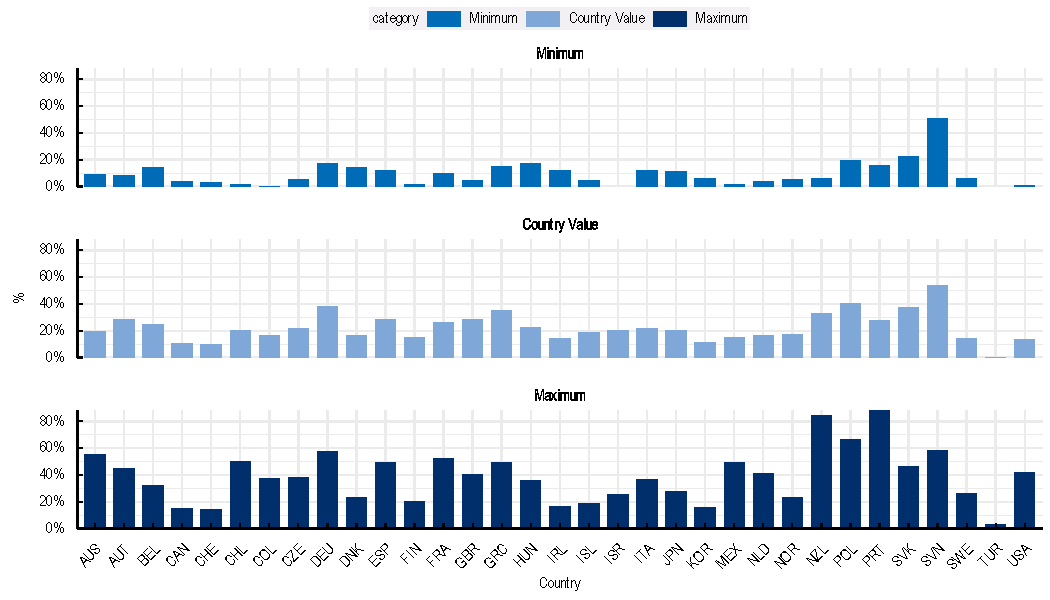
\includegraphics{book_figures/bar_final-1} \end{center}

\hypertarget{basic-graph}{%
\section{Basic graph}\label{basic-graph}}

You can use fonts such as Arial Narrow within \texttt{ggplot2}. This
package allows that with a dedicated function. The first thing to do is
load in the libraries and data, as below:

\begin{Shaded}
\begin{Highlighting}[]
\FunctionTok{library}\NormalTok{(oecdplot)}
\FunctionTok{library}\NormalTok{(ggplot2)}

\FunctionTok{load\_oecd\_fonts}\NormalTok{()}
\end{Highlighting}
\end{Shaded}

We will be working with the \texttt{pta} dataset, which is included in
the package.

\begin{Shaded}
\begin{Highlighting}[]
\NormalTok{pta}
\end{Highlighting}
\end{Shaded}

\begin{verbatim}
# A tibble: 99 x 4
   country region        category      pct_pta
   <fct>   <fct>         <fct>           <dbl>
 1 NZL     Auckland      Minimum          5.77
 2 NZL     Country Value Country Value   33.0 
 3 NZL     West Coast    Maximum         84.6 
 4 PRT     Centro        Minimum         15.6 
 5 PRT     Country Value Country Value   28.0 
 6 PRT     Algarve       Maximum         88.1 
 7 CHL     Coquimbo      Minimum          1.3 
 8 CHL     Country Value Country Value   20.5 
 9 CHL     Aysén         Maximum         49.8 
10 MEX     Guerrero      Minimum          1.47
# ... with 89 more rows
\end{verbatim}

To initialise a plot we tell ggplot that \texttt{pta} is our data, and
specify the variables on each axis. We then instruct ggplot to render
this as an bar plot by adding the \texttt{geom\_col()} function. The
\texttt{position} argument makes the categories appear side-by-side,
instead of stacking them on top of each other and the \texttt{width}
argument makes the columns thinner.

\begin{Shaded}
\begin{Highlighting}[]
\NormalTok{p }\OtherTok{\textless{}{-}} \FunctionTok{ggplot}\NormalTok{(}\AttributeTok{data =}\NormalTok{ pta, }\FunctionTok{aes}\NormalTok{(}\AttributeTok{x =}\NormalTok{ country, }\AttributeTok{y =}\NormalTok{ pct\_pta }\SpecialCharTok{/} \DecValTok{100}\NormalTok{, }\AttributeTok{fill =}\NormalTok{ category)) }\SpecialCharTok{+}
  \FunctionTok{geom\_col}\NormalTok{(}\AttributeTok{position =} \StringTok{"dodge2"}\NormalTok{, }\AttributeTok{width =} \FloatTok{0.7}\NormalTok{)}
\NormalTok{p}
\end{Highlighting}
\end{Shaded}

\begin{center}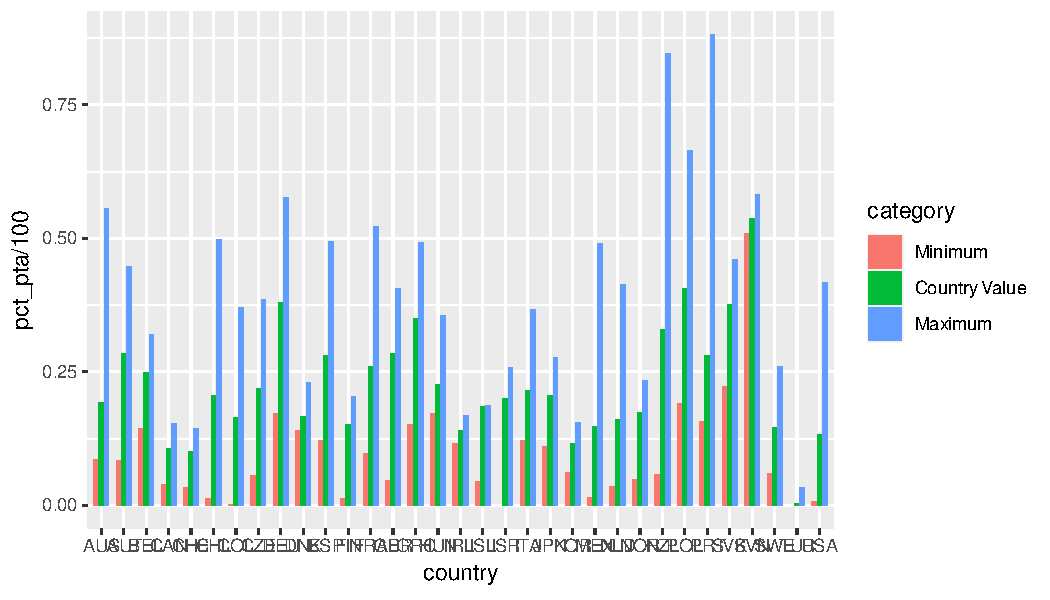
\includegraphics{book_figures/bar_1-1} \end{center}

\hypertarget{adjusting-theme}{%
\section{Adjusting theme}\label{adjusting-theme}}

We can change the overall look of the graph using themes. We'll start
using a simple theme customisation by adding \texttt{theme\_oecd()}
after \texttt{ggplot()}.

\begin{Shaded}
\begin{Highlighting}[]
\NormalTok{p }\OtherTok{\textless{}{-}}\NormalTok{ p }\SpecialCharTok{+}
  \FunctionTok{theme\_oecd}\NormalTok{()}
\NormalTok{p}
\end{Highlighting}
\end{Shaded}

\begin{center}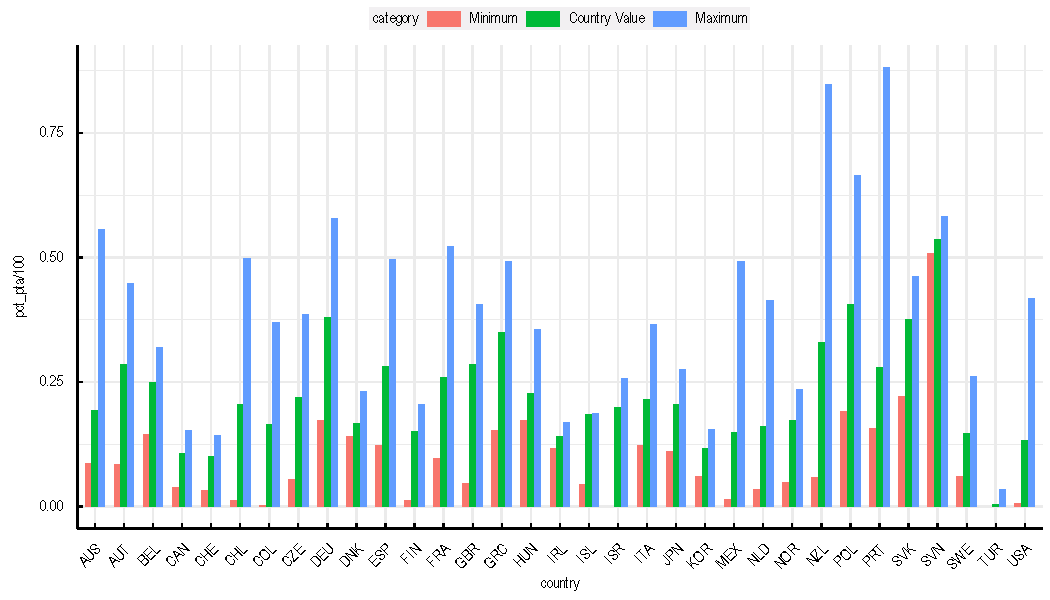
\includegraphics{book_figures/bar_2-1} \end{center}

\hypertarget{adjusting-color-palette}{%
\section{Adjusting color palette}\label{adjusting-color-palette}}

To change the colours, we use the OECD scales. Note that you can
reference the specific colours you'd like to use with specific HEX
codes. You can also reference colours by name, with the full list of
colours recognised by R
\href{http://www.stat.columbia.edu/~tzheng/files/Rcolor.pdf}{here}. Here
we are using some arguments inside the scale function, in order to show
some of the personalization alternatives.

\begin{Shaded}
\begin{Highlighting}[]
\NormalTok{p }\OtherTok{\textless{}{-}}\NormalTok{ p }\SpecialCharTok{+}
  \FunctionTok{scale\_fill\_oecd\_d}\NormalTok{(}\AttributeTok{option =} \StringTok{"darkblue"}\NormalTok{, }\AttributeTok{direction =} \SpecialCharTok{{-}}\DecValTok{1}\NormalTok{)}
\NormalTok{p}
\end{Highlighting}
\end{Shaded}

\begin{center}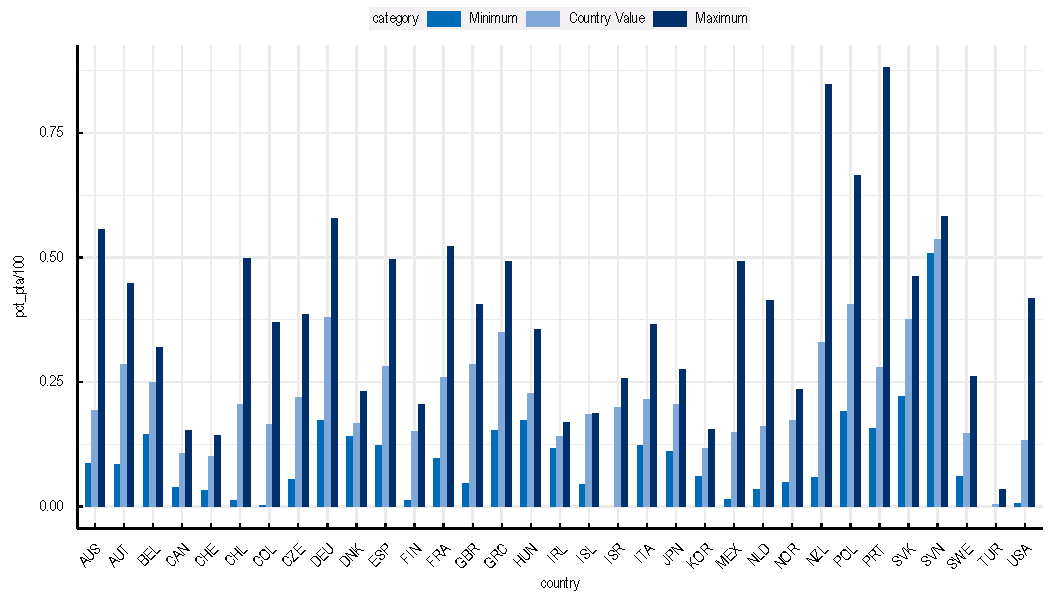
\includegraphics{book_figures/bar_3-1} \end{center}

\hypertarget{adjusting-axis-scale}{%
\section{Adjusting axis scale}\label{adjusting-axis-scale}}

To change the scale to percentage, we can use the \texttt{percent()}
function from the \texttt{scales} package, which comes with
\texttt{ggplot2}.

\begin{Shaded}
\begin{Highlighting}[]
\NormalTok{p }\OtherTok{\textless{}{-}}\NormalTok{ p }\SpecialCharTok{+}
  \FunctionTok{scale\_y\_continuous}\NormalTok{(}\AttributeTok{labels =}\NormalTok{ scales}\SpecialCharTok{::}\NormalTok{percent, }\AttributeTok{expand =} \FunctionTok{c}\NormalTok{(}\DecValTok{0}\NormalTok{,}\DecValTok{0}\NormalTok{))}
\NormalTok{p}
\end{Highlighting}
\end{Shaded}

\begin{center}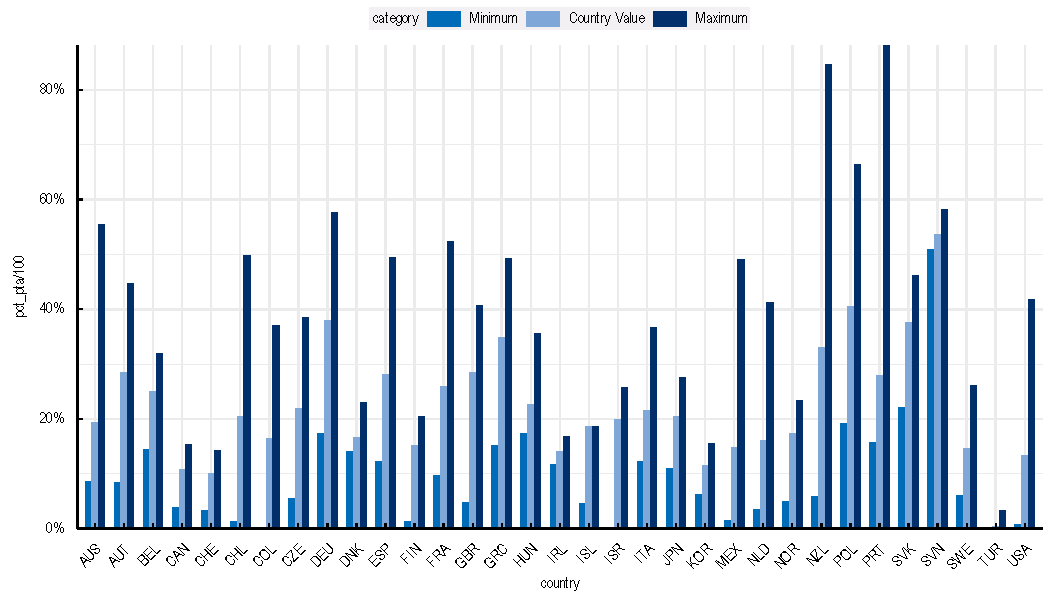
\includegraphics{book_figures/bar_4-1} \end{center}

\hypertarget{facetting}{%
\section{Facetting}\label{facetting}}

In order to divide the resulting plot into a 3-in-1 plot, we use the
\texttt{facet\_wrap()} function. The \texttt{ncol} argument is used to
arrange the resulting plots in one column, instead of creating a three
columns layout in this case.

\begin{Shaded}
\begin{Highlighting}[]
\NormalTok{p }\OtherTok{\textless{}{-}}\NormalTok{ p }\SpecialCharTok{+}
  \FunctionTok{facet\_wrap}\NormalTok{(}\SpecialCharTok{\textasciitilde{}}\NormalTok{category, }\AttributeTok{ncol =} \DecValTok{1}\NormalTok{)}
\NormalTok{p}
\end{Highlighting}
\end{Shaded}

\begin{center}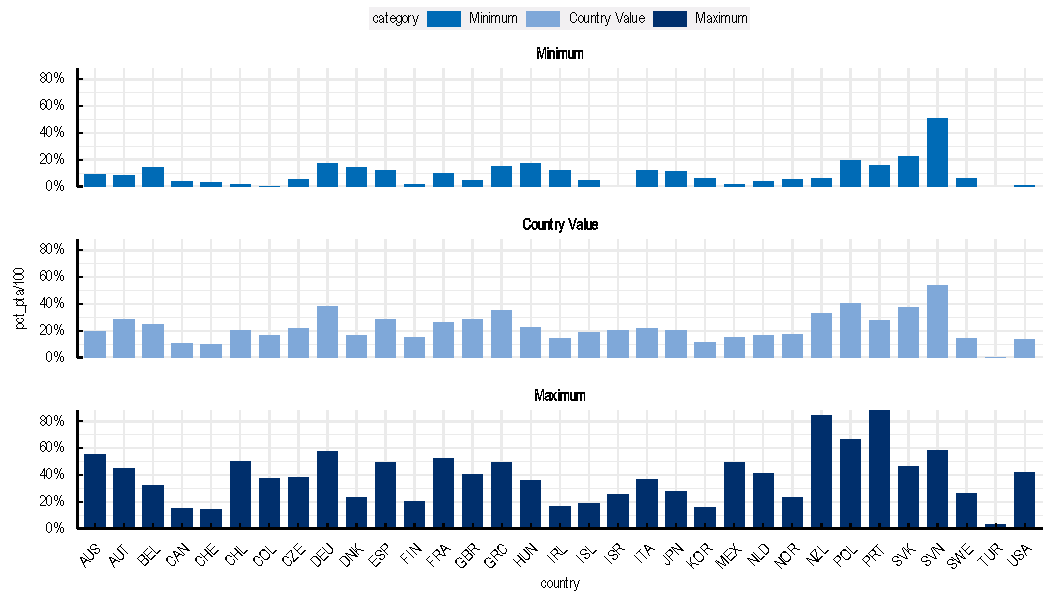
\includegraphics{book_figures/bar_5-1} \end{center}

\hypertarget{adding-labels}{%
\section{Adding labels}\label{adding-labels}}

To obtain the plot from the start of this section, we use the
\texttt{labs()} function.

\begin{Shaded}
\begin{Highlighting}[]
\NormalTok{p }\OtherTok{\textless{}{-}}\NormalTok{ p }\SpecialCharTok{+}
  \FunctionTok{labs}\NormalTok{(}
    \AttributeTok{x =} \StringTok{"Country"}\NormalTok{,}
    \AttributeTok{y =} \StringTok{"\%"}
\NormalTok{  )}
\NormalTok{p}
\end{Highlighting}
\end{Shaded}

\begin{center}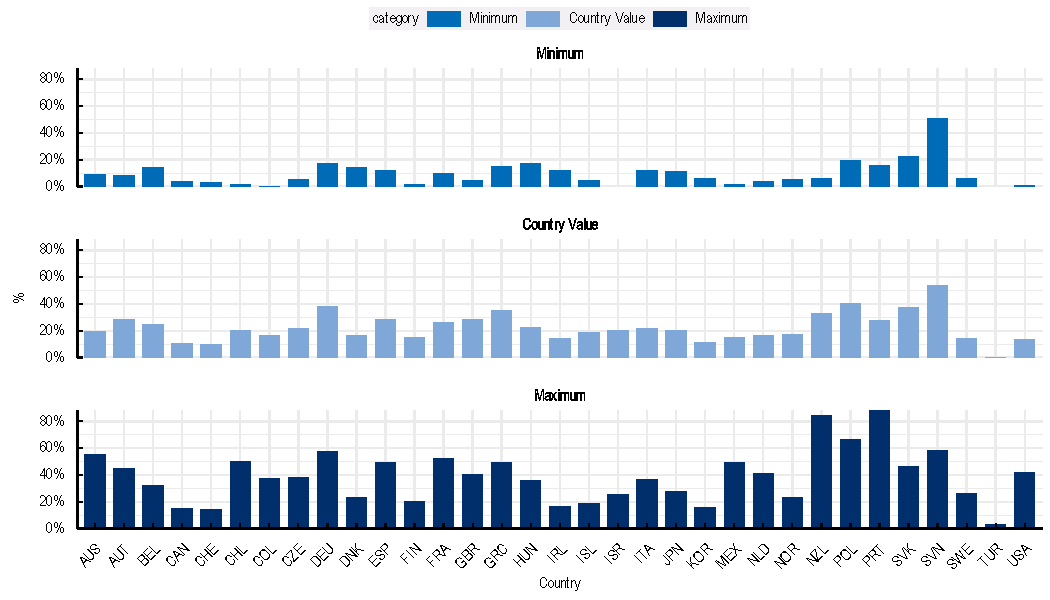
\includegraphics{book_figures/bar_6-1} \end{center}

\hypertarget{scatter-plots}{%
\chapter{Scatter plots}\label{scatter-plots}}

We will work towards creating the area plot below. We will take you from
a basic bar plot and explain all the customisations we add to the code
step-by-step.

\begin{center}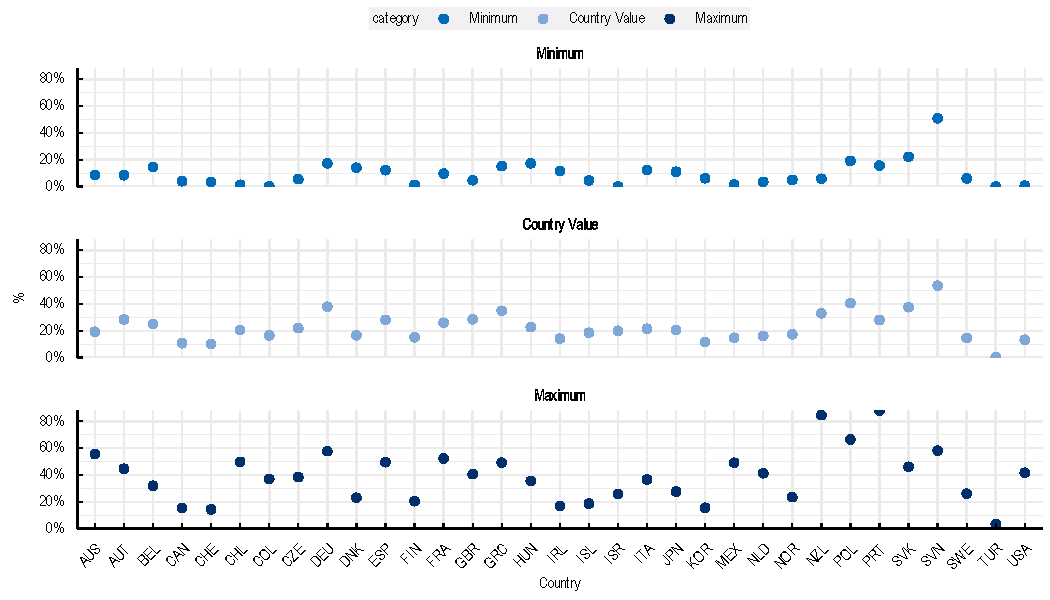
\includegraphics{book_figures/scatterplot_final-1} \end{center}

\hypertarget{basic-graph-1}{%
\section{Basic graph}\label{basic-graph-1}}

You can use fonts such as Arial Narrow within \texttt{ggplot2}. This
package allows that with a dedicated function. The first thing to do is
load in the libraries and data, as below:

\begin{Shaded}
\begin{Highlighting}[]
\FunctionTok{library}\NormalTok{(oecdplot)}
\FunctionTok{library}\NormalTok{(ggplot2)}

\FunctionTok{load\_oecd\_fonts}\NormalTok{()}
\end{Highlighting}
\end{Shaded}

We will be working with the \texttt{pta} dataset, which is included in
the package.

\begin{Shaded}
\begin{Highlighting}[]
\NormalTok{pta}
\end{Highlighting}
\end{Shaded}

\begin{verbatim}
# A tibble: 99 x 4
   country region        category      pct_pta
   <fct>   <fct>         <fct>           <dbl>
 1 NZL     Auckland      Minimum          5.77
 2 NZL     Country Value Country Value   33.0 
 3 NZL     West Coast    Maximum         84.6 
 4 PRT     Centro        Minimum         15.6 
 5 PRT     Country Value Country Value   28.0 
 6 PRT     Algarve       Maximum         88.1 
 7 CHL     Coquimbo      Minimum          1.3 
 8 CHL     Country Value Country Value   20.5 
 9 CHL     Aysén         Maximum         49.8 
10 MEX     Guerrero      Minimum          1.47
# ... with 89 more rows
\end{verbatim}

To initialise a plot we tell ggplot that \texttt{pta} is our data, and
specify the variables on each axis. We then instruct ggplot to render
this as an bar plot by adding the \texttt{geom\_col()} function. The
\texttt{position} argument makes the categories appear side-by-side,
instead of stacking them on top of each other.

\begin{Shaded}
\begin{Highlighting}[]
\NormalTok{p }\OtherTok{\textless{}{-}} \FunctionTok{ggplot}\NormalTok{(}\AttributeTok{data =}\NormalTok{ pta, }\FunctionTok{aes}\NormalTok{(}\AttributeTok{x =}\NormalTok{ country, }\AttributeTok{y =}\NormalTok{ pct\_pta }\SpecialCharTok{/} \DecValTok{100}\NormalTok{, }\AttributeTok{colour =}\NormalTok{ category)) }\SpecialCharTok{+}
  \FunctionTok{geom\_point}\NormalTok{(}\AttributeTok{position =} \StringTok{"dodge2"}\NormalTok{)}
\NormalTok{p}
\end{Highlighting}
\end{Shaded}

\begin{center}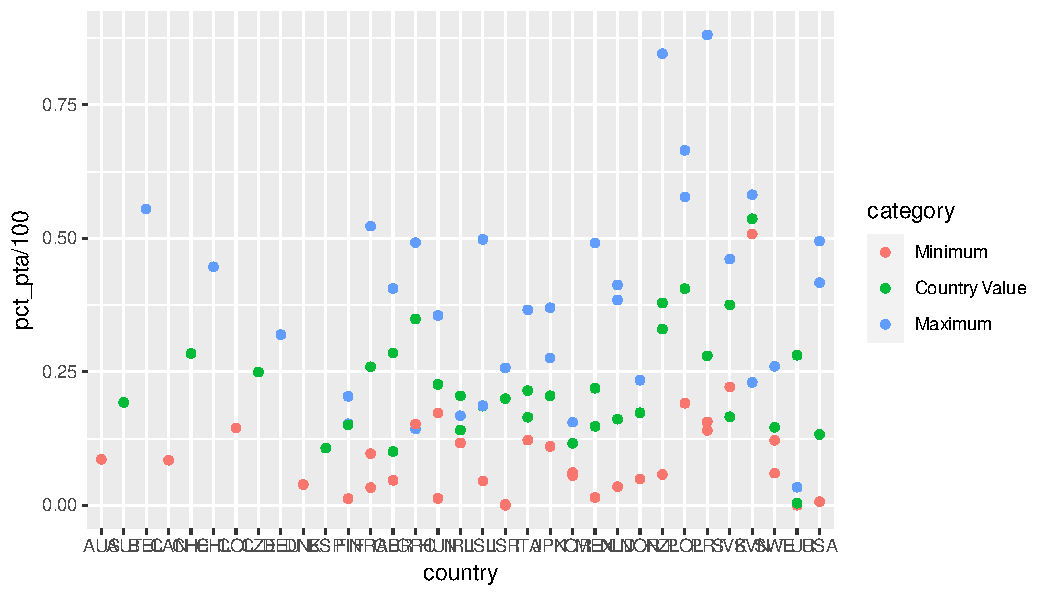
\includegraphics{book_figures/scatterplot_1-1} \end{center}

\hypertarget{adjusting-theme-1}{%
\section{Adjusting theme}\label{adjusting-theme-1}}

We can change the overall look of the graph using themes. We'll start
using a simple theme customisation by adding \texttt{theme\_oecd()}
after \texttt{ggplot()}.

\begin{Shaded}
\begin{Highlighting}[]
\NormalTok{p }\OtherTok{\textless{}{-}}\NormalTok{ p }\SpecialCharTok{+}
  \FunctionTok{theme\_oecd}\NormalTok{()}
\NormalTok{p}
\end{Highlighting}
\end{Shaded}

\begin{center}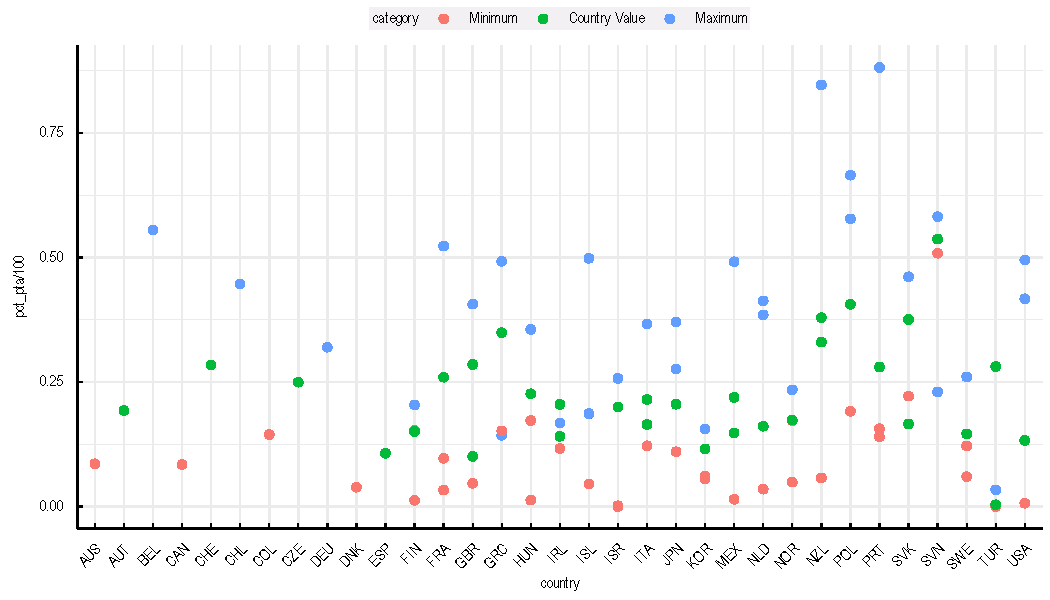
\includegraphics{book_figures/scatterplot_2-1} \end{center}

\hypertarget{adjusting-color-palette-1}{%
\section{Adjusting color palette}\label{adjusting-color-palette-1}}

To change the colours, we use the OECD scales. Note that you can
reference the specific colours you'd like to use with specific HEX
codes. You can also reference colours by name, with the full list of
colours recognised by R
\href{http://www.stat.columbia.edu/~tzheng/files/Rcolor.pdf}{here}. Here
we are using some arguments inside the scale function, in order to show
some of the personalization alternatives.

\begin{Shaded}
\begin{Highlighting}[]
\NormalTok{p }\OtherTok{\textless{}{-}}\NormalTok{ p }\SpecialCharTok{+}
  \FunctionTok{scale\_colour\_oecd\_d}\NormalTok{(}\AttributeTok{option =} \StringTok{"darkblue"}\NormalTok{, }\AttributeTok{direction =} \SpecialCharTok{{-}}\DecValTok{1}\NormalTok{)}
\NormalTok{p}
\end{Highlighting}
\end{Shaded}

\begin{center}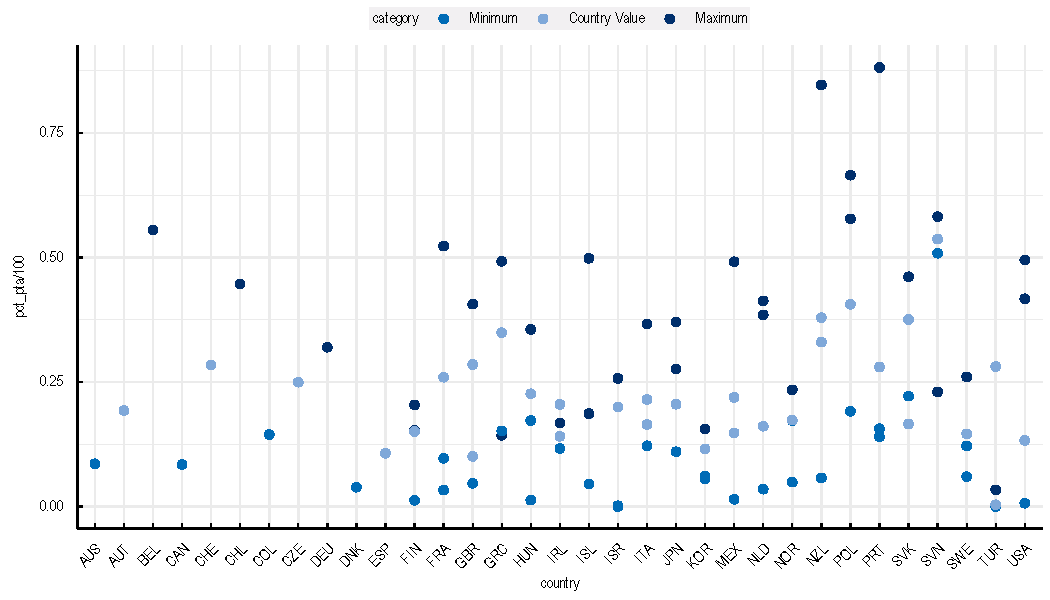
\includegraphics{book_figures/scatterplot_3-1} \end{center}

\hypertarget{adjusting-axis-scale-1}{%
\section{Adjusting axis scale}\label{adjusting-axis-scale-1}}

To change the scale to percentage, we can use the \texttt{percent()}
function from the \texttt{scales} package, which comes with
\texttt{ggplot2}.

\begin{Shaded}
\begin{Highlighting}[]
\NormalTok{p }\OtherTok{\textless{}{-}}\NormalTok{ p }\SpecialCharTok{+}
  \FunctionTok{scale\_y\_continuous}\NormalTok{(}\AttributeTok{labels =}\NormalTok{ scales}\SpecialCharTok{::}\NormalTok{percent, }\AttributeTok{expand =} \FunctionTok{c}\NormalTok{(}\DecValTok{0}\NormalTok{,}\DecValTok{0}\NormalTok{))}
\NormalTok{p}
\end{Highlighting}
\end{Shaded}

\begin{center}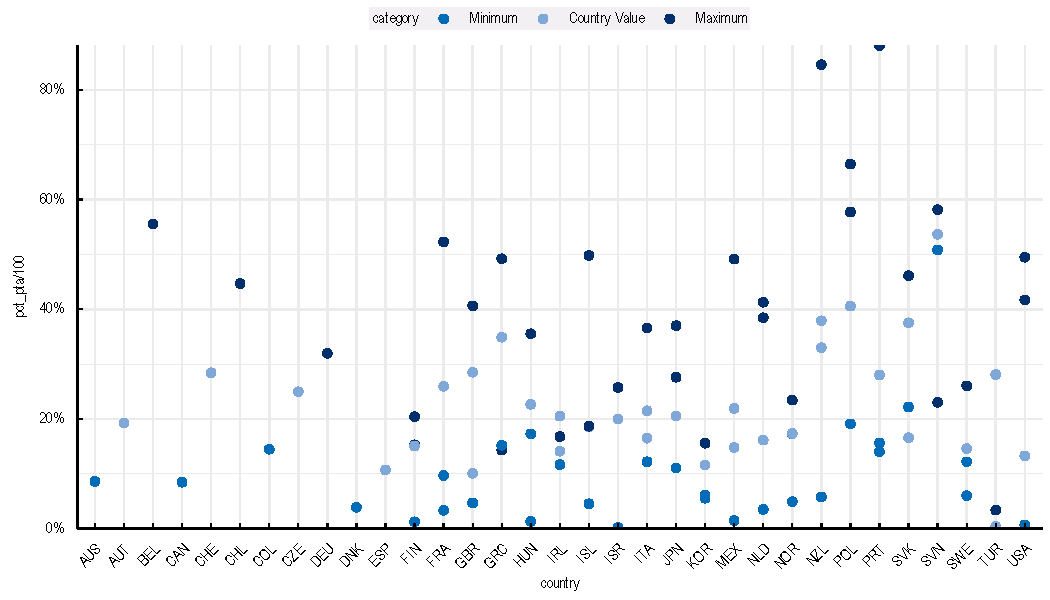
\includegraphics{book_figures/scatterplot_4-1} \end{center}

\hypertarget{facetting-1}{%
\section{Facetting}\label{facetting-1}}

In order to divide the resulting plot into a 3-in-1 plot, we use the
\texttt{facet\_wrap()} function. The \texttt{ncol} argument is used to
arrange the resulting plots in one column, instead of creating a three
columns layout in this case.

\begin{Shaded}
\begin{Highlighting}[]
\NormalTok{p }\OtherTok{\textless{}{-}}\NormalTok{ p }\SpecialCharTok{+}
  \FunctionTok{facet\_wrap}\NormalTok{(}\SpecialCharTok{\textasciitilde{}}\NormalTok{category, }\AttributeTok{ncol =} \DecValTok{1}\NormalTok{)}
\NormalTok{p}
\end{Highlighting}
\end{Shaded}

\begin{center}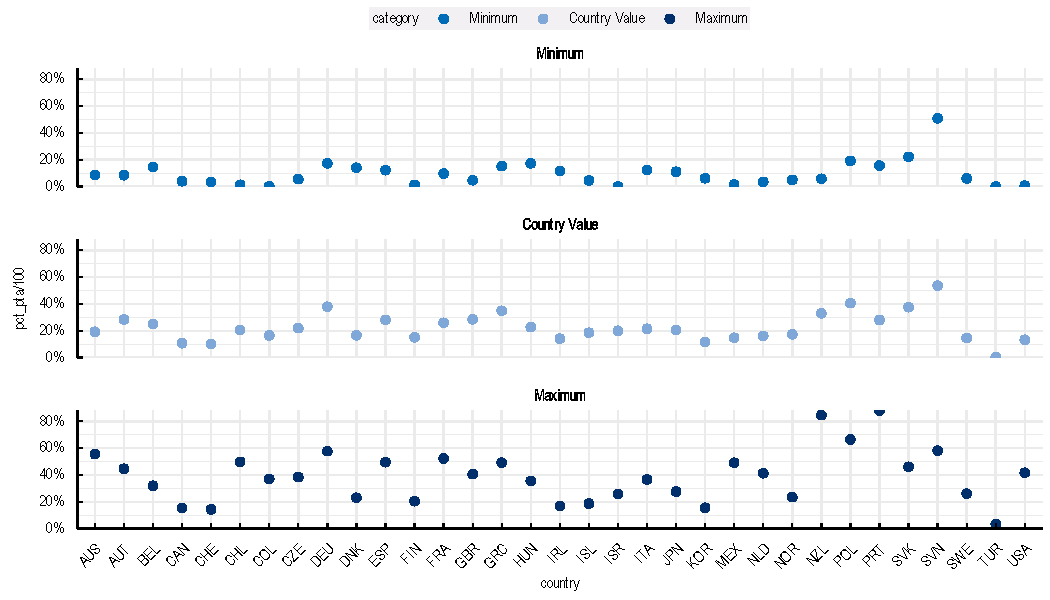
\includegraphics{book_figures/scatterplot_5-1} \end{center}

\hypertarget{adding-labels-1}{%
\section{Adding labels}\label{adding-labels-1}}

To obtain the plot from the start of this section, we use the
\texttt{labs()} function.

\begin{Shaded}
\begin{Highlighting}[]
\NormalTok{p }\OtherTok{\textless{}{-}}\NormalTok{ p }\SpecialCharTok{+}
  \FunctionTok{labs}\NormalTok{(}
    \AttributeTok{x =} \StringTok{"Country"}\NormalTok{,}
    \AttributeTok{y =} \StringTok{"\%"}
\NormalTok{  )}
\NormalTok{p}
\end{Highlighting}
\end{Shaded}

\begin{center}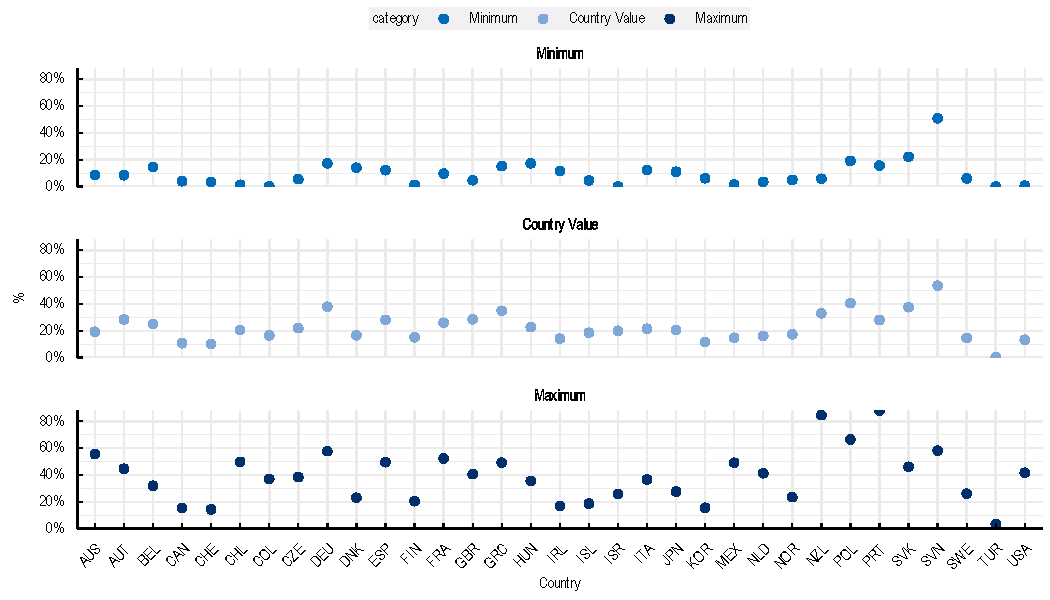
\includegraphics{book_figures/scatterplot_6-1} \end{center}

\hypertarget{min-max-plots}{%
\chapter{Min-max plots}\label{min-max-plots}}

We will work towards creating the area plot below. We will take you from
a basic bar plot and explain all the customisations we add to the code
step-by-step.

This plot is build by adding \emph{layers} of different geoms, using the
\texttt{geom\_line()} and \texttt{geom\_point()} functions. The first
one add the vertical grey line behind the dots, and the second adds the
overlaying points. Defining the shape parameter here adds a visual aid
to make it easier to differentiate the different values.

\begin{center}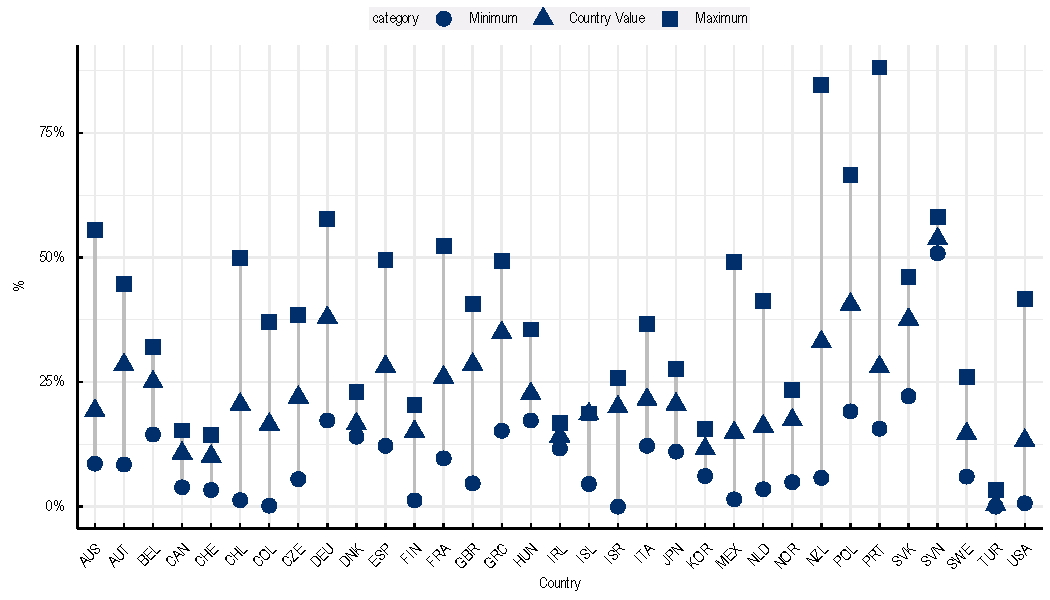
\includegraphics{book_figures/maxmin_final-1} \end{center}

\hypertarget{basic-graph-2}{%
\section{Basic graph}\label{basic-graph-2}}

You can use fonts such as Arial Narrow within \texttt{ggplot2}. This
package allows that with a dedicated function. The first thing to do is
load in the libraries and data, as below:

\begin{Shaded}
\begin{Highlighting}[]
\FunctionTok{library}\NormalTok{(oecdplot)}
\FunctionTok{library}\NormalTok{(ggplot2)}

\FunctionTok{load\_oecd\_fonts}\NormalTok{()}
\end{Highlighting}
\end{Shaded}

We will be working with the \texttt{pta} dataset, which is included in
the package.

\begin{Shaded}
\begin{Highlighting}[]
\NormalTok{pta}
\end{Highlighting}
\end{Shaded}

\begin{verbatim}
# A tibble: 99 x 4
   country region        category      pct_pta
   <fct>   <fct>         <fct>           <dbl>
 1 NZL     Auckland      Minimum          5.77
 2 NZL     Country Value Country Value   33.0 
 3 NZL     West Coast    Maximum         84.6 
 4 PRT     Centro        Minimum         15.6 
 5 PRT     Country Value Country Value   28.0 
 6 PRT     Algarve       Maximum         88.1 
 7 CHL     Coquimbo      Minimum          1.3 
 8 CHL     Country Value Country Value   20.5 
 9 CHL     Aysén         Maximum         49.8 
10 MEX     Guerrero      Minimum          1.47
# ... with 89 more rows
\end{verbatim}

To initialise a plot we tell ggplot that \texttt{pta} is our data, and
specify the variables on each axis. We then instruct ggplot to render
this as an bar plot by adding the \texttt{geom\_line()} and
\texttt{geom\_point()} functions. The colour argument is outside
\texttt{aes()} in order to use the same colour for each figure.

\begin{Shaded}
\begin{Highlighting}[]
\NormalTok{p }\OtherTok{\textless{}{-}} \FunctionTok{ggplot}\NormalTok{(pta, }\FunctionTok{aes}\NormalTok{(}\AttributeTok{x =}\NormalTok{ country, }\AttributeTok{y =}\NormalTok{ pct\_pta }\SpecialCharTok{/} \DecValTok{100}\NormalTok{)) }\SpecialCharTok{+}
  \FunctionTok{geom\_line}\NormalTok{(}\AttributeTok{colour =} \StringTok{"grey20"}\NormalTok{) }\SpecialCharTok{+}
  \FunctionTok{geom\_point}\NormalTok{(}
    \FunctionTok{aes}\NormalTok{(}\AttributeTok{shape =}\NormalTok{ category),}
    \AttributeTok{colour =} \FunctionTok{oecd\_clrs}\NormalTok{(}\AttributeTok{n =} \DecValTok{1}\NormalTok{, }\AttributeTok{option =} \StringTok{"darkblue"}\NormalTok{),}
    \AttributeTok{size =} \DecValTok{3}
\NormalTok{  )}
\NormalTok{p}
\end{Highlighting}
\end{Shaded}

\begin{center}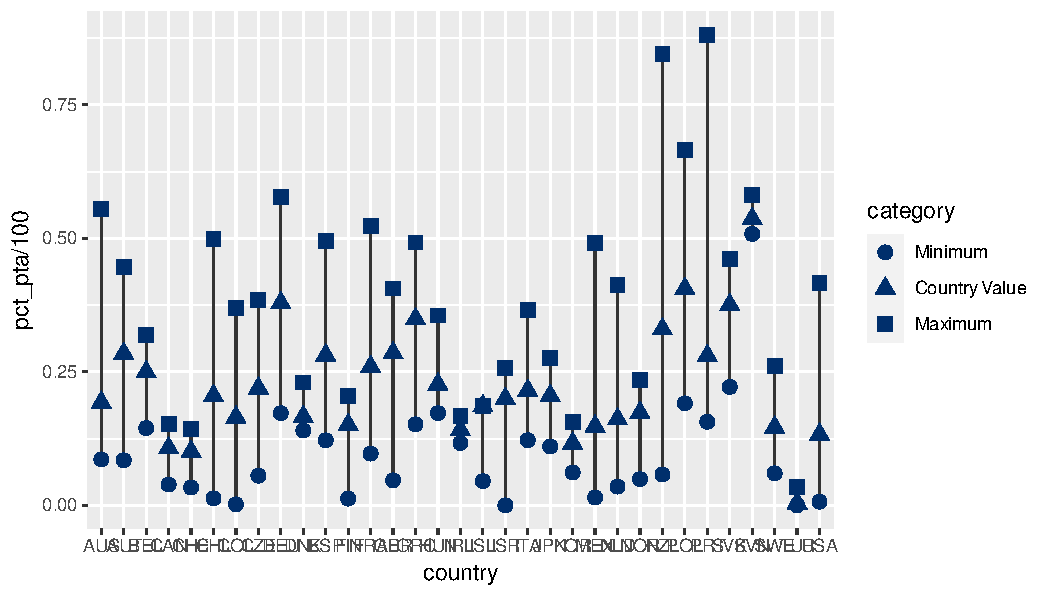
\includegraphics{book_figures/maxmin_1-1} \end{center}

\hypertarget{adjusting-theme-2}{%
\section{Adjusting theme}\label{adjusting-theme-2}}

We can change the overall look of the graph using themes. We'll start
using a simple theme customisation by adding \texttt{theme\_oecd()}
after \texttt{ggplot()}.

\begin{Shaded}
\begin{Highlighting}[]
\NormalTok{p }\OtherTok{\textless{}{-}}\NormalTok{ p }\SpecialCharTok{+}
  \FunctionTok{theme\_oecd}\NormalTok{()}
\NormalTok{p}
\end{Highlighting}
\end{Shaded}

\begin{center}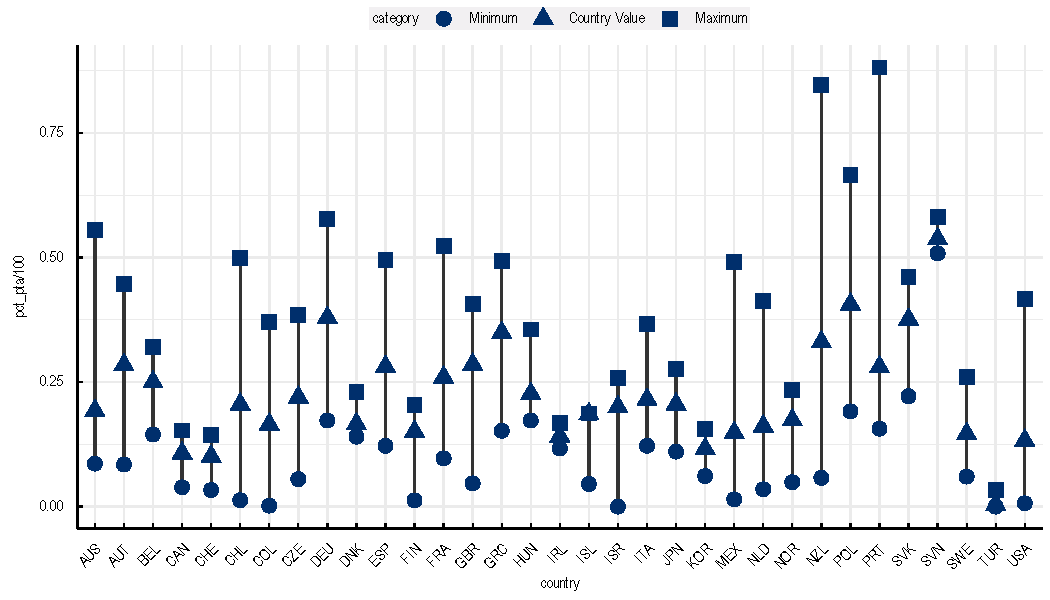
\includegraphics{book_figures/maxmin_2-1} \end{center}

\hypertarget{adjusting-axis-scale-2}{%
\section{Adjusting axis scale}\label{adjusting-axis-scale-2}}

To change the scale to percentage, we can use the \texttt{percent()}
function from the \texttt{scales} package, which comes with
\texttt{ggplot2}.

\begin{Shaded}
\begin{Highlighting}[]
\NormalTok{p }\OtherTok{\textless{}{-}}\NormalTok{ p }\SpecialCharTok{+}
  \FunctionTok{scale\_y\_continuous}\NormalTok{(}
    \AttributeTok{labels =}\NormalTok{ scales}\SpecialCharTok{::}\NormalTok{percent,}
    \AttributeTok{expand =} \FunctionTok{c}\NormalTok{(}\DecValTok{0}\NormalTok{,}\DecValTok{0}\NormalTok{),}
    \AttributeTok{limits =} \FunctionTok{c}\NormalTok{(}\DecValTok{0}\NormalTok{,}\DecValTok{1}\NormalTok{)}
\NormalTok{  )}
\NormalTok{p}
\end{Highlighting}
\end{Shaded}

\begin{center}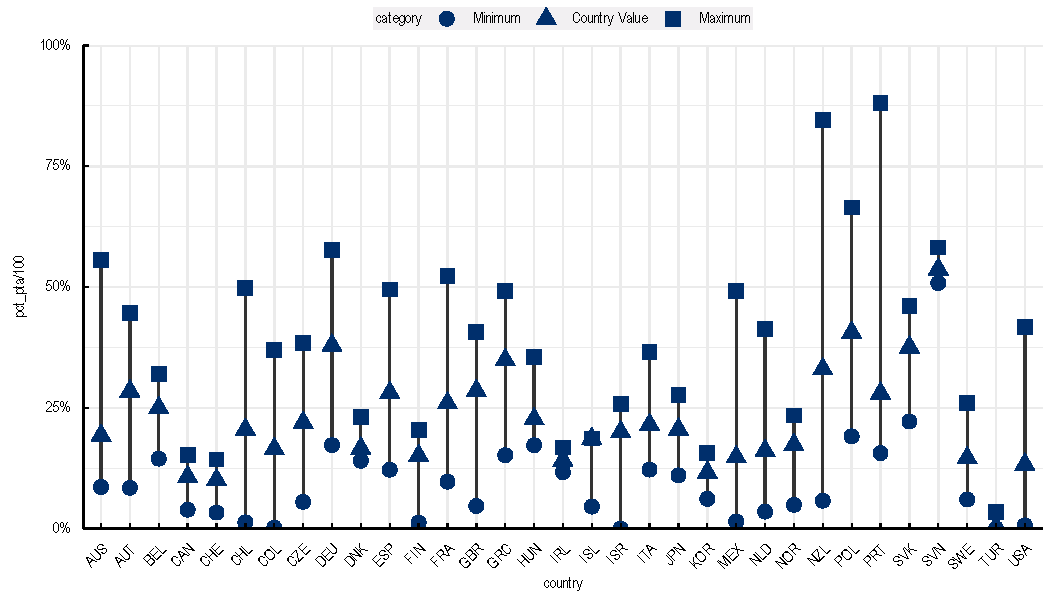
\includegraphics{book_figures/maxmin_3-1} \end{center}

\hypertarget{adding-labels-2}{%
\section{Adding labels}\label{adding-labels-2}}

To obtain the plot from the start of this section, we use the
\texttt{labs()} function.

\begin{Shaded}
\begin{Highlighting}[]
\NormalTok{p }\OtherTok{\textless{}{-}}\NormalTok{ p }\SpecialCharTok{+}
  \FunctionTok{labs}\NormalTok{(}
    \AttributeTok{x =} \StringTok{"Country"}\NormalTok{,}
    \AttributeTok{y =} \StringTok{"\%"}
\NormalTok{  )}
\NormalTok{p}
\end{Highlighting}
\end{Shaded}

\begin{center}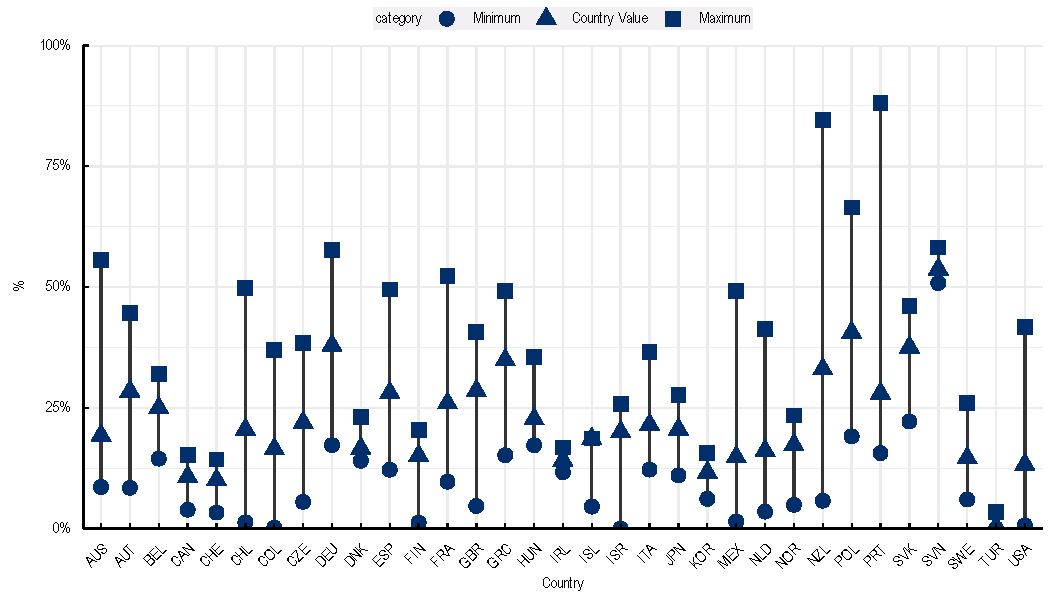
\includegraphics{book_figures/maxmin_4-1} \end{center}

\hypertarget{shortcuts}{%
\chapter{Shortcuts}\label{shortcuts}}

We will work towards creating different plots by using shortcut
functions within this package.

\hypertarget{column-plot}{%
\section{Column plot}\label{column-plot}}

Simple column plot:

\begin{Shaded}
\begin{Highlighting}[]
\FunctionTok{oecd\_col}\NormalTok{(}\AttributeTok{data =}\NormalTok{ pta, }\AttributeTok{x =}\NormalTok{ country, }\AttributeTok{y =}\NormalTok{ pct\_pta,  }\AttributeTok{colour =}\NormalTok{ category)}
\end{Highlighting}
\end{Shaded}

\begin{center}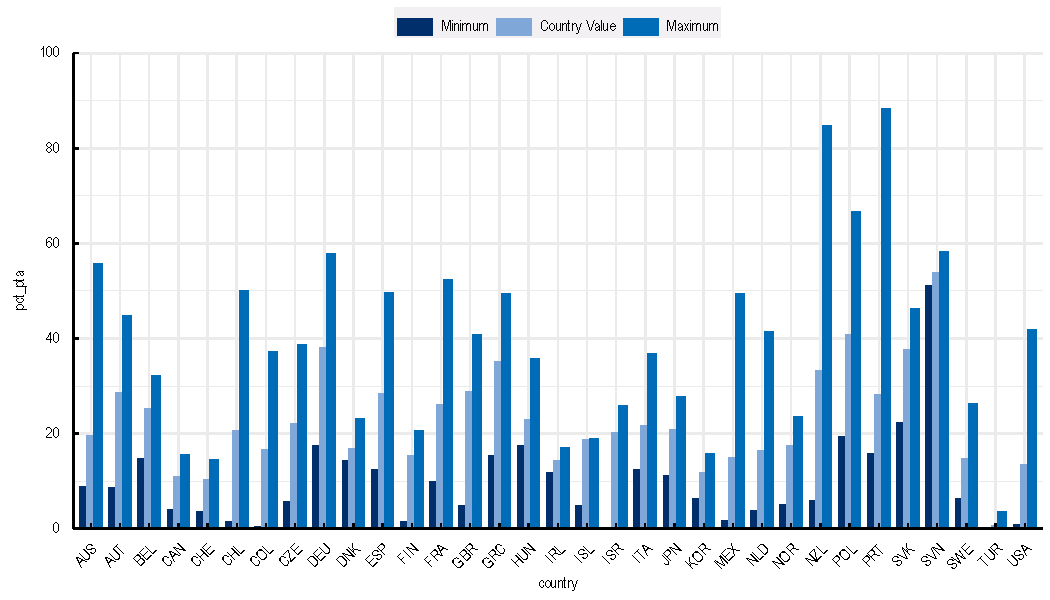
\includegraphics{book_figures/sc1-1} \end{center}

Stacked column plot:

\begin{Shaded}
\begin{Highlighting}[]
\FunctionTok{oecd\_col}\NormalTok{(}\AttributeTok{data =}\NormalTok{ pta, }\AttributeTok{x =}\NormalTok{ country, }\AttributeTok{y =}\NormalTok{ pct\_pta, }\AttributeTok{colour =}\NormalTok{ category, }\AttributeTok{stacked =}\NormalTok{ T)}
\end{Highlighting}
\end{Shaded}

\begin{center}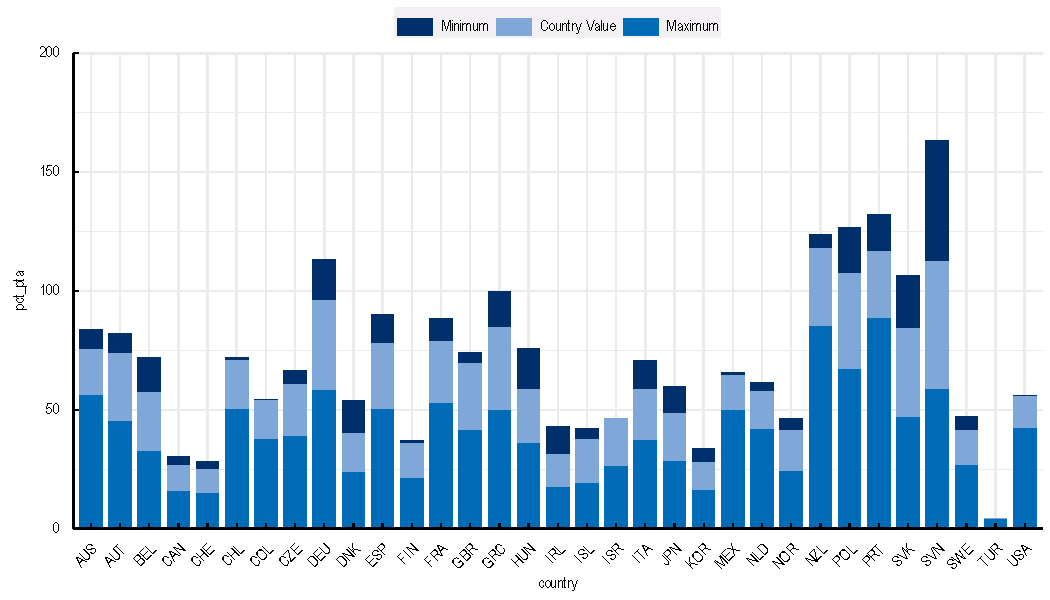
\includegraphics{book_figures/sc2-1} \end{center}

Stacked column plot with y-axis as percentage:

\begin{Shaded}
\begin{Highlighting}[]
\NormalTok{pta2 }\OtherTok{\textless{}{-}}\NormalTok{ pta}
\NormalTok{pta2}\SpecialCharTok{$}\NormalTok{pct\_pta }\OtherTok{\textless{}{-}}\NormalTok{ pta2}\SpecialCharTok{$}\NormalTok{pct\_pta }\SpecialCharTok{/} \DecValTok{100}
\FunctionTok{oecd\_col}\NormalTok{(}\AttributeTok{data =}\NormalTok{ pta2, }\AttributeTok{x =}\NormalTok{ country, }\AttributeTok{y =}\NormalTok{ pct\_pta, }\AttributeTok{colour =}\NormalTok{ category) }\SpecialCharTok{+}
  \FunctionTok{scale\_y\_continuous}\NormalTok{(}\AttributeTok{labels =}\NormalTok{ scales}\SpecialCharTok{::}\NormalTok{percent, }\AttributeTok{expand =} \FunctionTok{c}\NormalTok{(}\DecValTok{0}\NormalTok{,}\DecValTok{0}\NormalTok{))}
\end{Highlighting}
\end{Shaded}

\begin{center}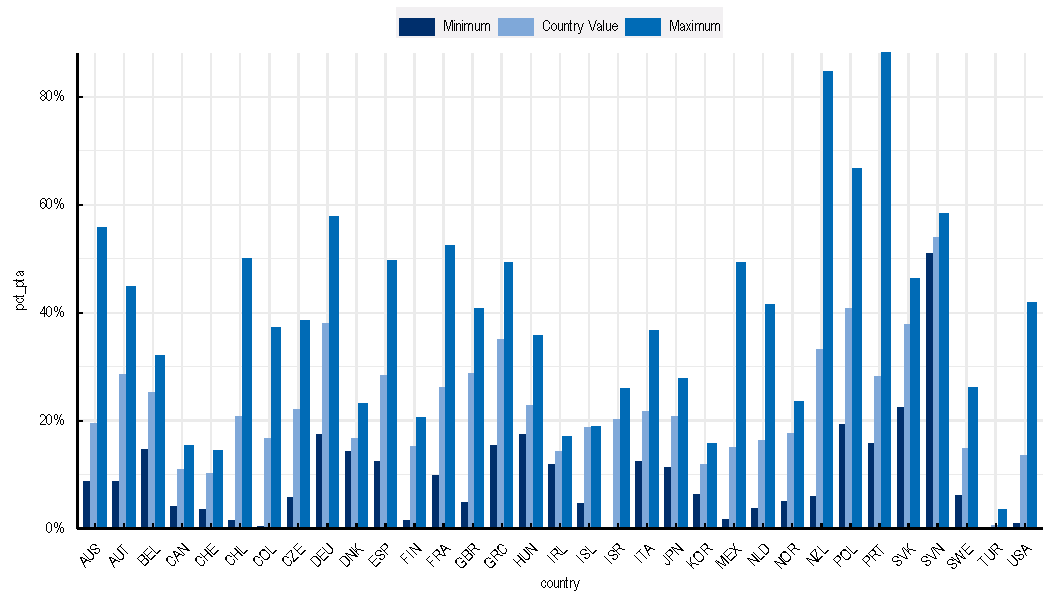
\includegraphics{book_figures/sc3-1} \end{center}

Faceted column plot with y-axis as percentage:

\begin{Shaded}
\begin{Highlighting}[]
\NormalTok{pta2 }\OtherTok{\textless{}{-}}\NormalTok{ pta}
\NormalTok{pta2}\SpecialCharTok{$}\NormalTok{pct\_pta }\OtherTok{\textless{}{-}}\NormalTok{ pta2}\SpecialCharTok{$}\NormalTok{pct\_pta }\SpecialCharTok{/} \DecValTok{100}

\FunctionTok{oecd\_col}\NormalTok{(}\AttributeTok{data =}\NormalTok{ pta2, }\AttributeTok{x =}\NormalTok{ country, }\AttributeTok{y =}\NormalTok{ pct\_pta, }\AttributeTok{colour =}\NormalTok{ category,}
         \AttributeTok{facet =}\NormalTok{ category) }\SpecialCharTok{+}
  \FunctionTok{scale\_y\_continuous}\NormalTok{(}\AttributeTok{labels =}\NormalTok{ scales}\SpecialCharTok{::}\NormalTok{percent, }\AttributeTok{expand =} \FunctionTok{c}\NormalTok{(}\DecValTok{0}\NormalTok{,}\DecValTok{0}\NormalTok{))}
\end{Highlighting}
\end{Shaded}

\begin{center}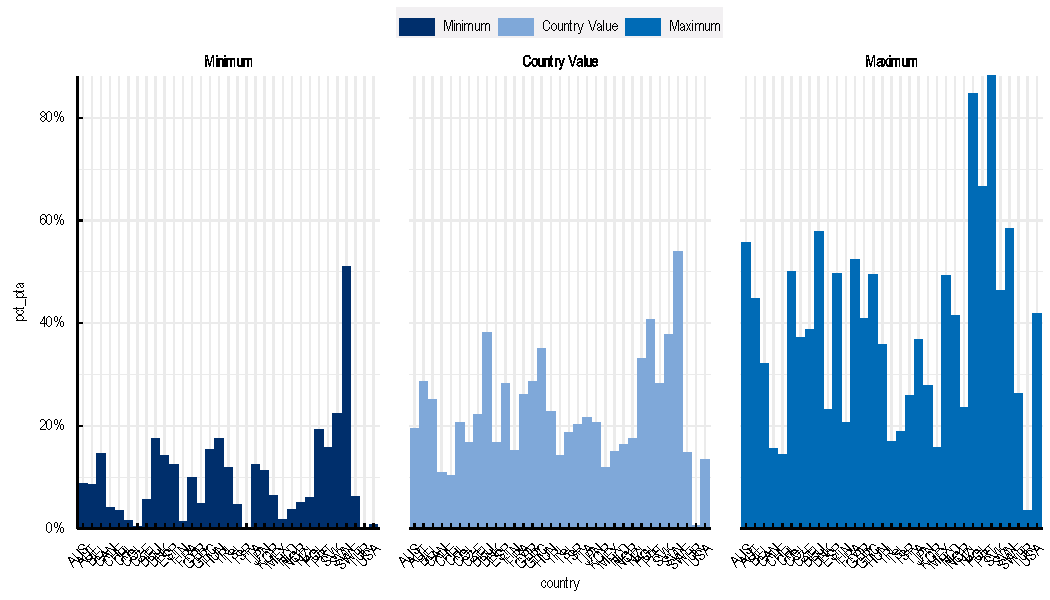
\includegraphics{book_figures/sc4-1} \end{center}

\hypertarget{line-plot}{%
\section{Line plot}\label{line-plot}}

Simple column plot:

\begin{Shaded}
\begin{Highlighting}[]
\FunctionTok{oecd\_line}\NormalTok{(pta, }\AttributeTok{x =}\NormalTok{ country, }\AttributeTok{y =}\NormalTok{ pct\_pta, }\AttributeTok{colour =}\NormalTok{ category, }\AttributeTok{group =}\NormalTok{ category)}
\end{Highlighting}
\end{Shaded}

\begin{center}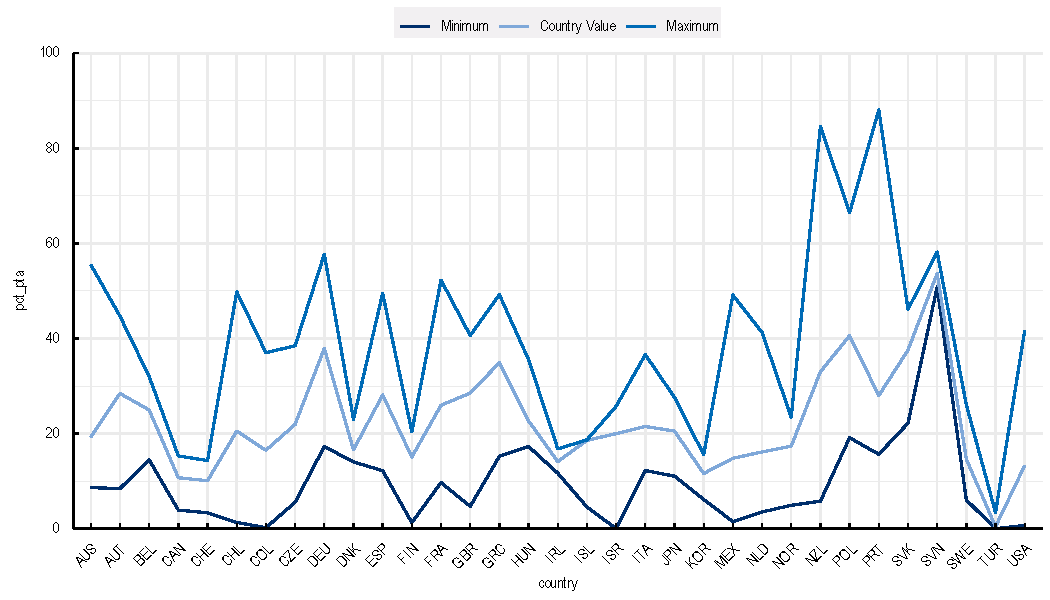
\includegraphics{book_figures/sl1-1} \end{center}

Faceted line plot:

\begin{Shaded}
\begin{Highlighting}[]
\FunctionTok{oecd\_line}\NormalTok{(pta,}
  \AttributeTok{x =}\NormalTok{ country, }\AttributeTok{y =}\NormalTok{ pct\_pta, }\AttributeTok{colour =}\NormalTok{ category, }\AttributeTok{group =}\NormalTok{ category,}
  \AttributeTok{facet =}\NormalTok{ category}
\NormalTok{)}
\end{Highlighting}
\end{Shaded}

\begin{center}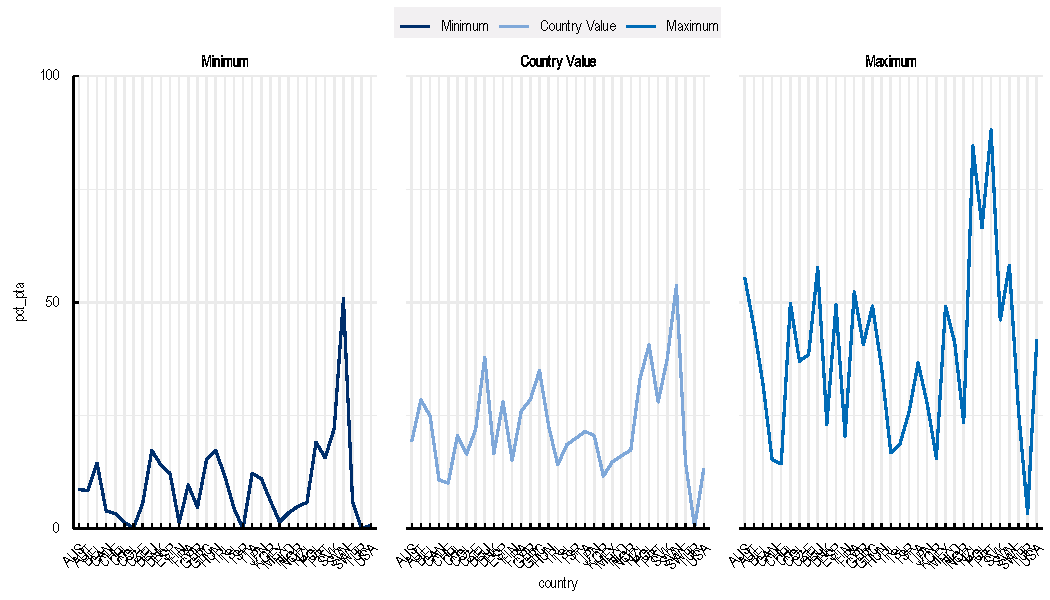
\includegraphics{book_figures/sl2-1} \end{center}

Faceted line plot with custom ordering:

\begin{Shaded}
\begin{Highlighting}[]
\FunctionTok{oecd\_line}\NormalTok{(pta,}
  \AttributeTok{x =}\NormalTok{ country, }\AttributeTok{y =}\NormalTok{ pct\_pta, }\AttributeTok{colour =}\NormalTok{ category, }\AttributeTok{group =}\NormalTok{ category,}
  \AttributeTok{facet =}\NormalTok{ category, }\AttributeTok{facet\_ncol =} \DecValTok{1}
\NormalTok{)}
\end{Highlighting}
\end{Shaded}

\begin{center}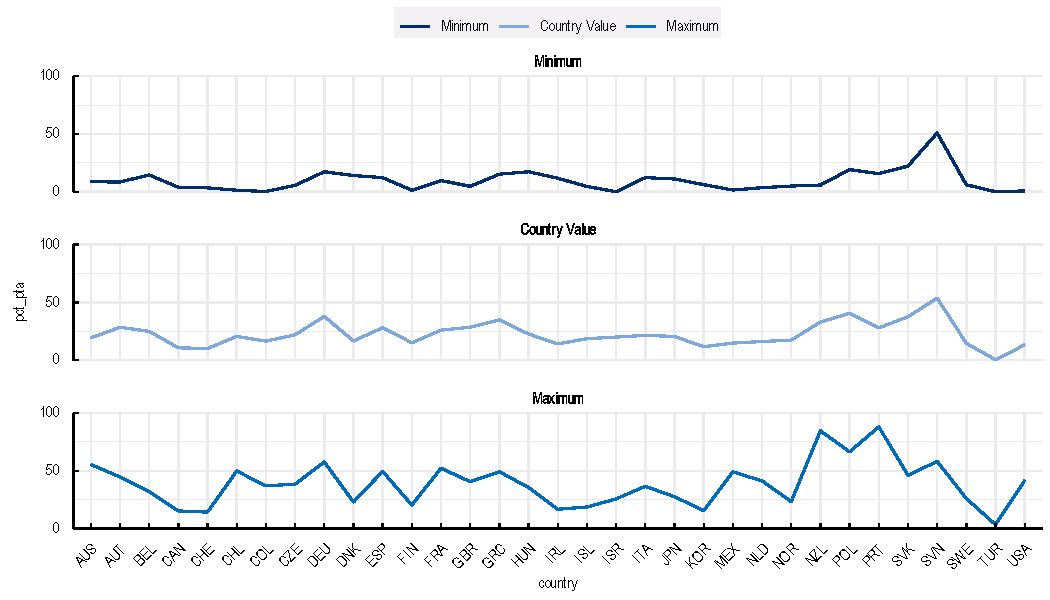
\includegraphics{book_figures/sl3-1} \end{center}

\hypertarget{scatterplot}{%
\section{Scatterplot}\label{scatterplot}}

Simple scatterplot:

\begin{Shaded}
\begin{Highlighting}[]
\FunctionTok{oecd\_point}\NormalTok{(pta, }\AttributeTok{x =}\NormalTok{ country, }\AttributeTok{y =}\NormalTok{ pct\_pta, }\AttributeTok{colour =}\NormalTok{ category, }\AttributeTok{group =}\NormalTok{ category)}
\end{Highlighting}
\end{Shaded}

\begin{center}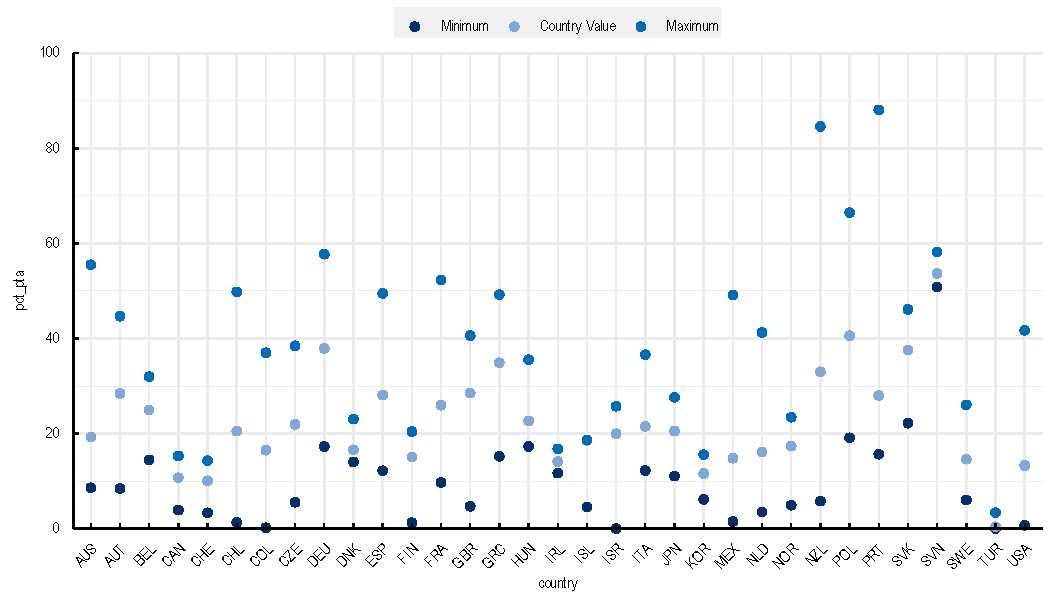
\includegraphics{book_figures/sp1-1} \end{center}

Faceted scatterplot:

\begin{Shaded}
\begin{Highlighting}[]
\FunctionTok{oecd\_point}\NormalTok{(pta,}
  \AttributeTok{x =}\NormalTok{ country, }\AttributeTok{y =}\NormalTok{ pct\_pta, }\AttributeTok{colour =}\NormalTok{ category, }\AttributeTok{group =}\NormalTok{ category,}
  \AttributeTok{facet =}\NormalTok{ category}
\NormalTok{)}
\end{Highlighting}
\end{Shaded}

\begin{center}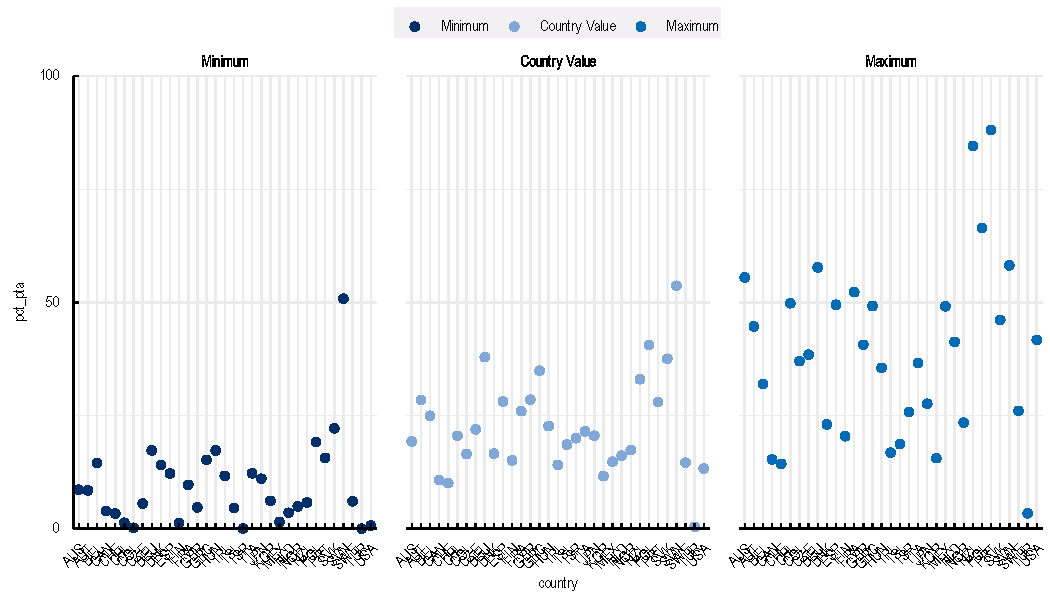
\includegraphics{book_figures/sp2-1} \end{center}

Faceted line plot with custom ordering:

\begin{Shaded}
\begin{Highlighting}[]
\FunctionTok{oecd\_point}\NormalTok{(pta,}
  \AttributeTok{x =}\NormalTok{ country, }\AttributeTok{y =}\NormalTok{ pct\_pta, }\AttributeTok{colour =}\NormalTok{ category, }\AttributeTok{group =}\NormalTok{ category,}
  \AttributeTok{facet =}\NormalTok{ category, }\AttributeTok{facet\_ncol =} \DecValTok{1}
\NormalTok{)}
\end{Highlighting}
\end{Shaded}

\begin{center}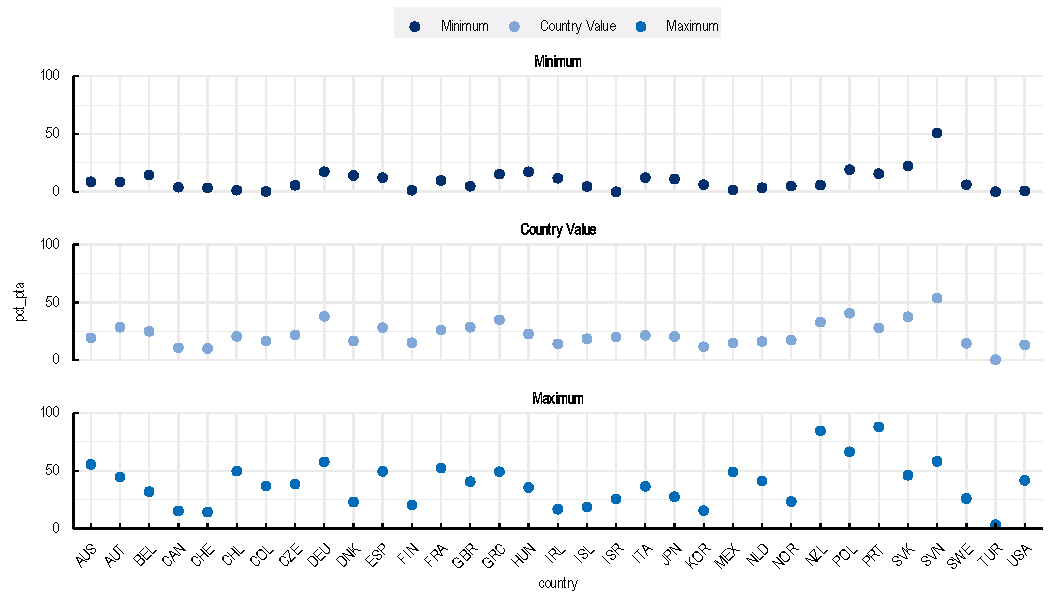
\includegraphics{book_figures/sp3-1} \end{center}

Options specific to scatterplots:

\begin{Shaded}
\begin{Highlighting}[]
\FunctionTok{oecd\_point}\NormalTok{(pta,}
  \AttributeTok{x =}\NormalTok{ country, }\AttributeTok{y =}\NormalTok{ pct\_pta, }\AttributeTok{colour =}\NormalTok{ category, }\AttributeTok{group =}\NormalTok{ category,}
  \AttributeTok{facet =}\NormalTok{ category, }\AttributeTok{facet\_ncol =} \DecValTok{1}\NormalTok{, }\AttributeTok{size =} \FunctionTok{log}\NormalTok{(pct\_pta)}
\NormalTok{)}
\end{Highlighting}
\end{Shaded}

\begin{center}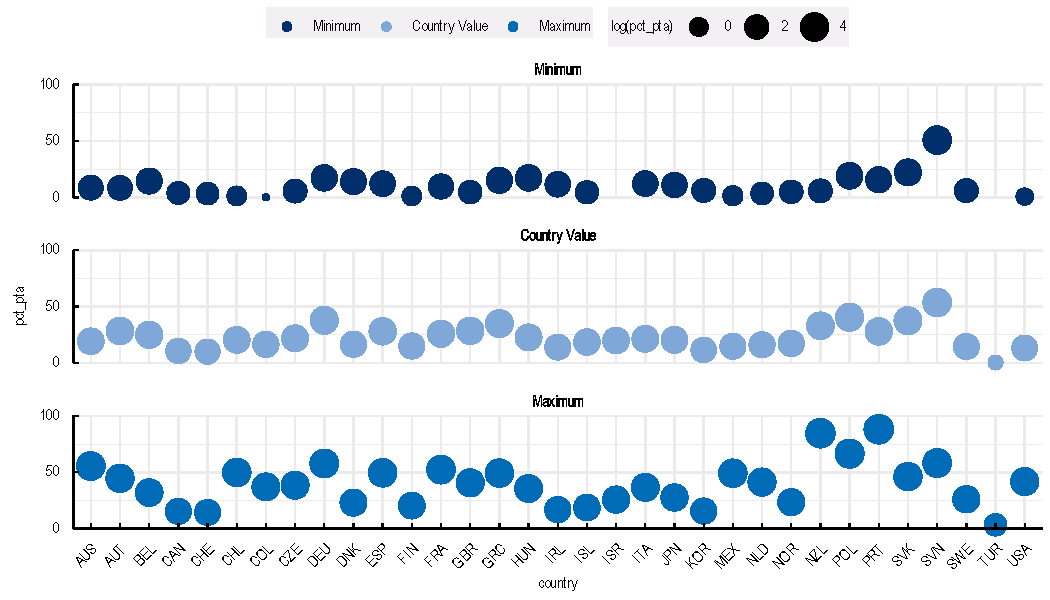
\includegraphics{book_figures/sp4-1} \end{center}

\hypertarget{max-min-plot}{%
\chapter{Max-min plot}\label{max-min-plot}}

Simple max-min plot:

\begin{Shaded}
\begin{Highlighting}[]
\FunctionTok{oecd\_maxmin}\NormalTok{(pta, }\AttributeTok{x =}\NormalTok{ country, }\AttributeTok{y =}\NormalTok{ pct\_pta, }\AttributeTok{colour =}\NormalTok{ category, }\AttributeTok{group =}\NormalTok{ category)}
\end{Highlighting}
\end{Shaded}

\begin{center}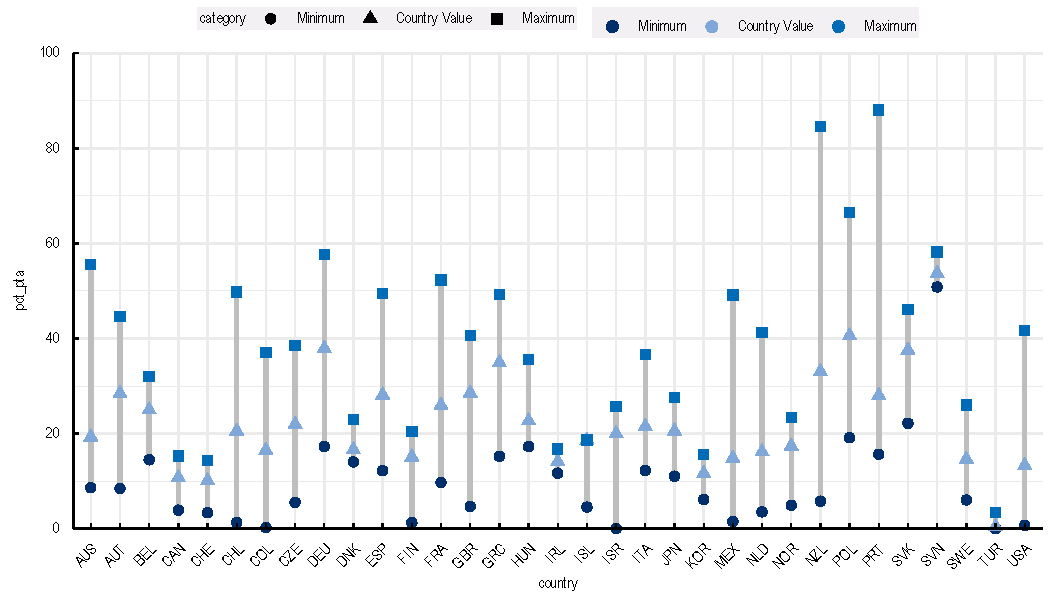
\includegraphics{book_figures/sm1-1} \end{center}

Faceted max-min plot:

\begin{Shaded}
\begin{Highlighting}[]
\FunctionTok{oecd\_maxmin}\NormalTok{(pta,}
  \AttributeTok{x =}\NormalTok{ country, }\AttributeTok{y =}\NormalTok{ pct\_pta, }\AttributeTok{colour =}\NormalTok{ category, }\AttributeTok{group =}\NormalTok{ category,}
  \AttributeTok{facet =}\NormalTok{ category}
\NormalTok{)}
\end{Highlighting}
\end{Shaded}

\begin{center}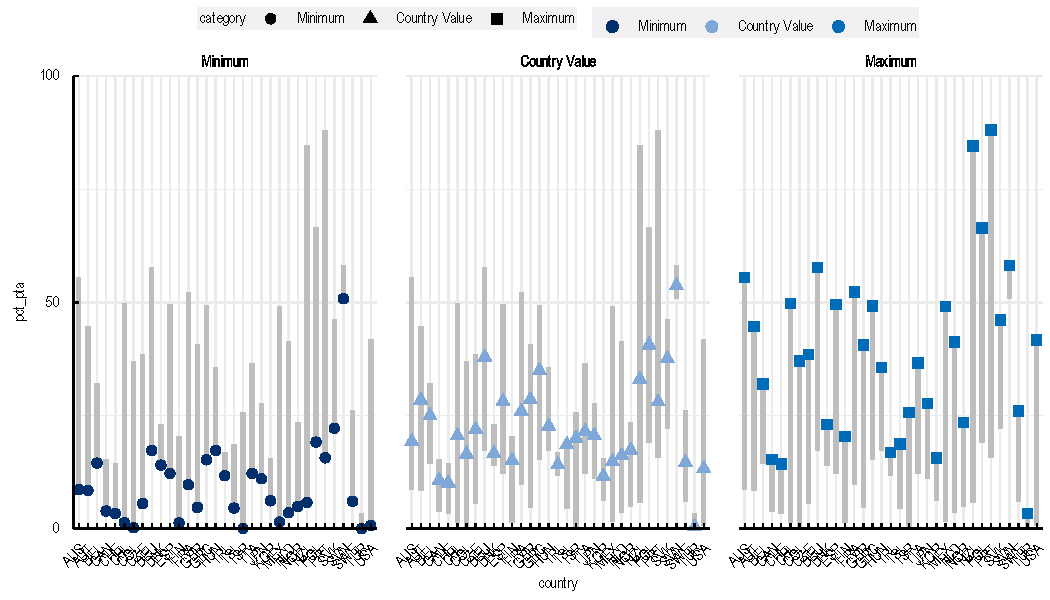
\includegraphics{book_figures/sm2-1} \end{center}

Faceted max-min plot with custom ordering:

\begin{Shaded}
\begin{Highlighting}[]
\FunctionTok{oecd\_maxmin}\NormalTok{(pta,}
  \AttributeTok{x =}\NormalTok{ country, }\AttributeTok{y =}\NormalTok{ pct\_pta, }\AttributeTok{colour =}\NormalTok{ category, }\AttributeTok{group =}\NormalTok{ category,}
  \AttributeTok{facet =}\NormalTok{ category, }\AttributeTok{facet\_ncol =} \DecValTok{1}
\NormalTok{)}
\end{Highlighting}
\end{Shaded}

\begin{center}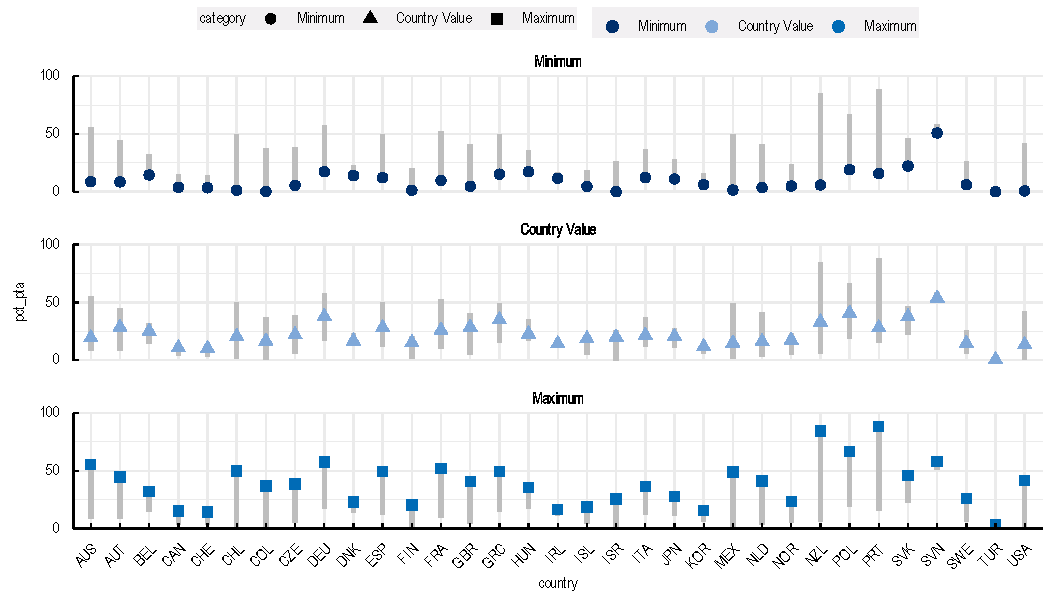
\includegraphics{book_figures/sm3-1} \end{center}

\hypertarget{what-if}{%
\chapter{What If?}\label{what-if}}

\hypertarget{exporting-plots-for-official-publication}{%
\section{Exporting plots for official
publication}\label{exporting-plots-for-official-publication}}

Suppose you have the next plot.

\begin{Shaded}
\begin{Highlighting}[]
\FunctionTok{library}\NormalTok{(ggplot2)}
\FunctionTok{library}\NormalTok{(oecdplot)}

\FunctionTok{load\_oecd\_fonts}\NormalTok{()}

\FunctionTok{ggplot}\NormalTok{(}\AttributeTok{data =}\NormalTok{ pta, }\FunctionTok{aes}\NormalTok{(}\AttributeTok{x =}\NormalTok{ country, }\AttributeTok{y =}\NormalTok{ pct\_pta }\SpecialCharTok{/} \DecValTok{100}\NormalTok{, }\AttributeTok{fill =}\NormalTok{ category)) }\SpecialCharTok{+}
  \FunctionTok{geom\_col}\NormalTok{(}\AttributeTok{position =} \StringTok{"dodge2"}\NormalTok{, }\AttributeTok{width =} \FloatTok{0.7}\NormalTok{) }\SpecialCharTok{+}
  \FunctionTok{theme\_oecd}\NormalTok{() }\SpecialCharTok{+}
  \FunctionTok{scale\_fill\_oecd\_d}\NormalTok{(}\AttributeTok{option =} \StringTok{"darkblue"}\NormalTok{, }\AttributeTok{direction =} \SpecialCharTok{{-}}\DecValTok{1}\NormalTok{) }\SpecialCharTok{+}
  \FunctionTok{scale\_y\_continuous}\NormalTok{(}\AttributeTok{labels =}\NormalTok{ scales}\SpecialCharTok{::}\NormalTok{percent, }\AttributeTok{expand =} \FunctionTok{c}\NormalTok{(}\DecValTok{0}\NormalTok{,}\DecValTok{0}\NormalTok{)) }\SpecialCharTok{+}
  \FunctionTok{facet\_wrap}\NormalTok{(}\SpecialCharTok{\textasciitilde{}}\NormalTok{category, }\AttributeTok{ncol =} \DecValTok{1}\NormalTok{) }\SpecialCharTok{+}
  \FunctionTok{labs}\NormalTok{(}
    \AttributeTok{x =} \StringTok{"Country"}\NormalTok{,}
    \AttributeTok{y =} \StringTok{"\%"}
\NormalTok{  )}
\end{Highlighting}
\end{Shaded}

\begin{center}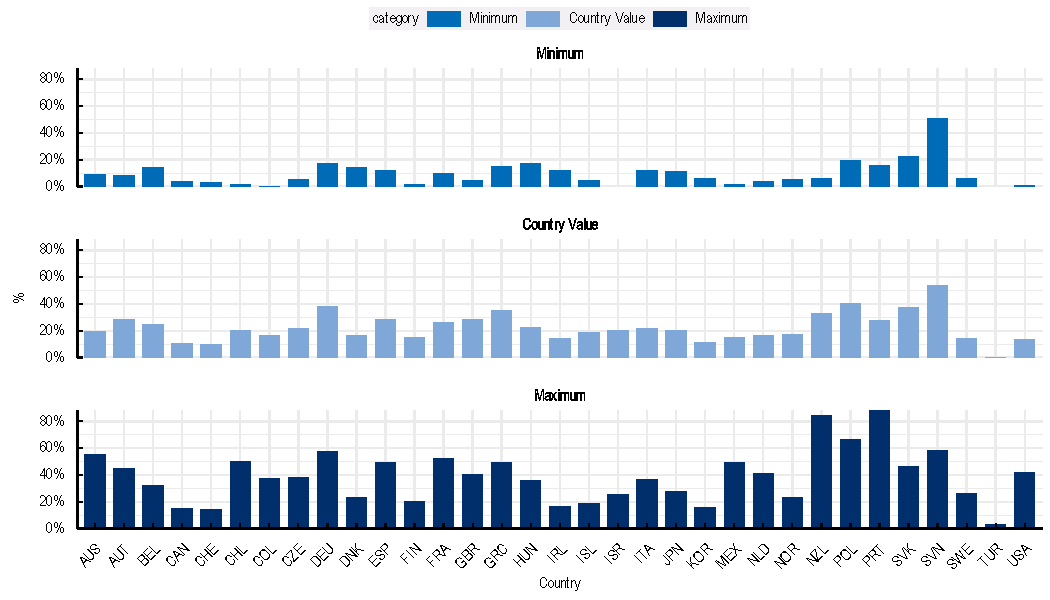
\includegraphics{book_figures/whatif_emf_1-1} \end{center}

We would only need to use the \texttt{save\_oecd\_chart()} function
which already provides PAC-compatible aesthetic elements including
dimensions and formats.

\begin{Shaded}
\begin{Highlighting}[]
\FunctionTok{save\_oecd\_chart}\NormalTok{(}
  \AttributeTok{file\_name =} \StringTok{"Figure 1"}\NormalTok{,}
  \AttributeTok{plot =} \FunctionTok{last\_plot}\NormalTok{(),}
  \AttributeTok{folder =} \StringTok{"my\_folder/"}\NormalTok{,}
  \AttributeTok{size =} \StringTok{"1/2"}\NormalTok{,}
  \AttributeTok{plot\_title =} \StringTok{"Figure 1. Regional disparities in protected terrestrial areas, 2017"}\NormalTok{,}
  \AttributeTok{plot\_note =} \StringTok{"Protected terrestrial areas refers to all protected areas recorded }
\StringTok{   in the World Database on Protected Areas (WDPA)"}\NormalTok{,}
  \AttributeTok{plot\_source =} \StringTok{"OECD calculations based World Database on Protected Areas (WDPA). }
\StringTok{   OECD (2020), OECD Regional Statistics (database)"}\NormalTok{,}
  \AttributeTok{statlink\_create =} \ConstantTok{TRUE}\NormalTok{,}
  \AttributeTok{statlink\_dataframe =}\NormalTok{ pta,}
  \AttributeTok{statlink\_filename =} \StringTok{"pta"}\NormalTok{,}
  \AttributeTok{box =} \ConstantTok{FALSE}\NormalTok{,}
  \AttributeTok{custom\_size =} \ConstantTok{NULL}\NormalTok{,}
  \AttributeTok{format =} \StringTok{"emf"}
\NormalTok{)}
\end{Highlighting}
\end{Shaded}

In the code above we can also pass \texttt{format\ =\ c("png","emf")} to
create two files at the same time.

\hypertarget{trailing-and-leading-spaces-in-the-plotting-area}{%
\section{Trailing and leading spaces in the plotting
area}\label{trailing-and-leading-spaces-in-the-plotting-area}}

Consider the next plot, where we already applied the OECD theme and
formatted the labels as percentage.

\begin{Shaded}
\begin{Highlighting}[]
\FunctionTok{library}\NormalTok{(dplyr)}
\FunctionTok{library}\NormalTok{(tidyr)}
\FunctionTok{library}\NormalTok{(ggplot2)}
\FunctionTok{library}\NormalTok{(oecdplot)}

\FunctionTok{load\_oecd\_fonts}\NormalTok{()}

\NormalTok{pta2 }\OtherTok{\textless{}{-}}\NormalTok{ pta }\SpecialCharTok{\%\textgreater{}\%} 
  \FunctionTok{filter}\NormalTok{(category }\SpecialCharTok{==} \StringTok{"Country Value"}\NormalTok{) }\SpecialCharTok{\%\textgreater{}\%} 
  \FunctionTok{mutate}\NormalTok{(}\AttributeTok{pct\_non\_pta =} \DecValTok{100} \SpecialCharTok{{-}}\NormalTok{ pct\_pta) }\SpecialCharTok{\%\textgreater{}\%} 
  \FunctionTok{pivot\_longer}\NormalTok{(pct\_pta}\SpecialCharTok{:}\NormalTok{pct\_non\_pta) }\SpecialCharTok{\%\textgreater{}\%} 
  \FunctionTok{mutate}\NormalTok{(}\AttributeTok{value =}\NormalTok{ value }\SpecialCharTok{/} \DecValTok{100}\NormalTok{)}

\NormalTok{pta2\_plot }\OtherTok{\textless{}{-}}\NormalTok{ pta2 }\SpecialCharTok{\%\textgreater{}\%}
  \FunctionTok{ggplot}\NormalTok{(}\FunctionTok{aes}\NormalTok{(}\AttributeTok{x =}\NormalTok{ value, }\AttributeTok{y =}\NormalTok{ country)) }\SpecialCharTok{+}
  \FunctionTok{geom\_col}\NormalTok{(}\FunctionTok{aes}\NormalTok{(}\AttributeTok{fill =}\NormalTok{ name), }\AttributeTok{width =} \FloatTok{0.4}\NormalTok{) }\SpecialCharTok{+}
  \FunctionTok{scale\_fill\_oecd\_d}\NormalTok{() }\SpecialCharTok{+}
  \FunctionTok{labs}\NormalTok{(}\AttributeTok{y =} \StringTok{"Country"}\NormalTok{, }\AttributeTok{x =} \StringTok{"\%"}\NormalTok{) }\SpecialCharTok{+}
  \FunctionTok{theme\_oecd}\NormalTok{(}\AttributeTok{base\_x\_axis\_angle =} \DecValTok{0}\NormalTok{)}\SpecialCharTok{+}
  \FunctionTok{scale\_x\_continuous}\NormalTok{(}
    \AttributeTok{labels =}\NormalTok{ scales}\SpecialCharTok{::}\FunctionTok{percent\_format}\NormalTok{(}\AttributeTok{accuracy =} \DecValTok{1}\NormalTok{)}
\NormalTok{  )}

\NormalTok{pta2\_plot}
\end{Highlighting}
\end{Shaded}

\begin{center}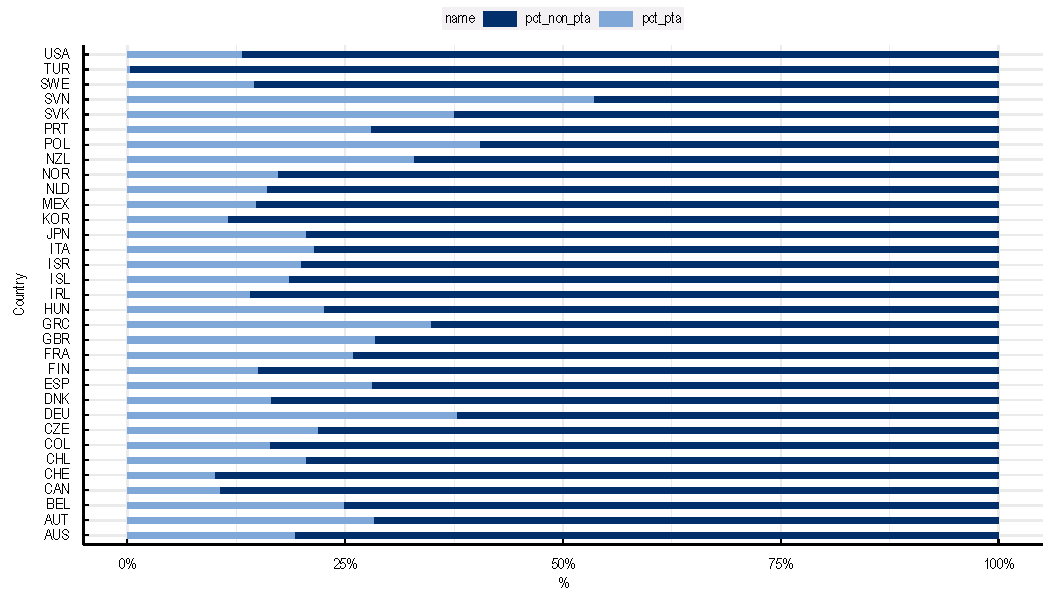
\includegraphics{book_figures/whatif_whitespace_1-1} \end{center}

One option to remove the whitespace in the plot is to use the
\texttt{expand} parameter, in order to start from the (0,0) coordinate.

\begin{Shaded}
\begin{Highlighting}[]
\NormalTok{pta2\_plot }\SpecialCharTok{+} 
  \FunctionTok{scale\_x\_continuous}\NormalTok{(}
    \AttributeTok{expand =} \FunctionTok{c}\NormalTok{(}\DecValTok{0}\NormalTok{,}\DecValTok{0}\NormalTok{),}
    \AttributeTok{labels =}\NormalTok{ scales}\SpecialCharTok{::}\FunctionTok{percent\_format}\NormalTok{(}\AttributeTok{accuracy =} \DecValTok{1}\NormalTok{)}
\NormalTok{  )}
\end{Highlighting}
\end{Shaded}

\begin{center}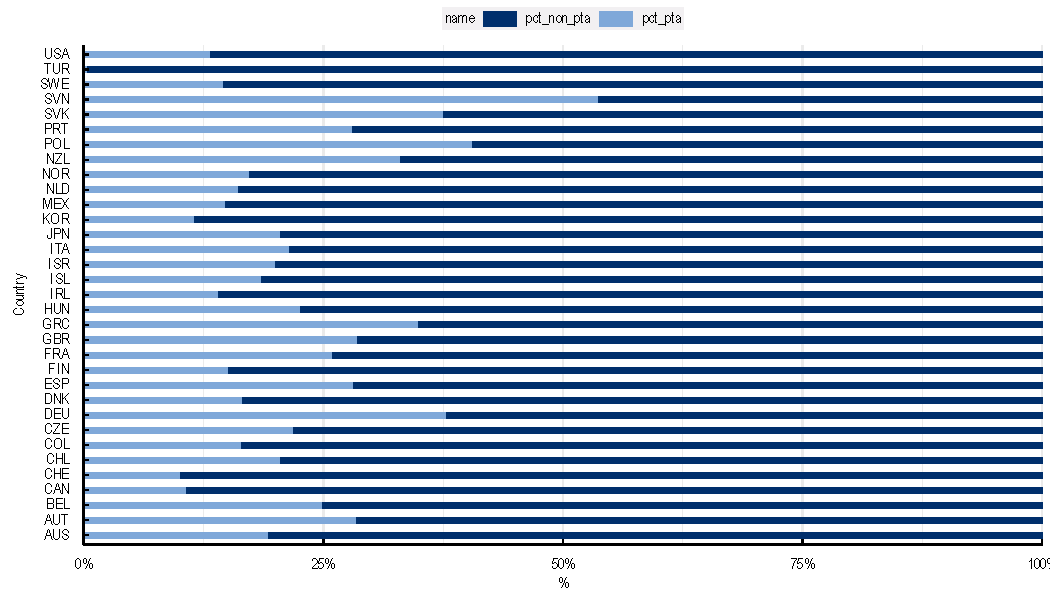
\includegraphics{book_figures/whatif_whitespace_2-1} \end{center}

This plot has a problem, the ``100\%'' label is outside the margins,
which is covered in then next what-if.

\hypertarget{the-x-axis-contains-off-margin-labels}{%
\section{The x-axis contains off-margin
labels}\label{the-x-axis-contains-off-margin-labels}}

Consider the next plot, where we added different adjustments, such as
the x-axis labels rotation.

\begin{Shaded}
\begin{Highlighting}[]
\FunctionTok{library}\NormalTok{(dplyr)}
\FunctionTok{library}\NormalTok{(tidyr)}
\FunctionTok{library}\NormalTok{(ggplot2)}
\FunctionTok{library}\NormalTok{(oecdplot)}

\FunctionTok{load\_oecd\_fonts}\NormalTok{()}

\NormalTok{pta2 }\OtherTok{\textless{}{-}}\NormalTok{ pta }\SpecialCharTok{\%\textgreater{}\%} 
  \FunctionTok{filter}\NormalTok{(category }\SpecialCharTok{==} \StringTok{"Country Value"}\NormalTok{) }\SpecialCharTok{\%\textgreater{}\%} 
  \FunctionTok{mutate}\NormalTok{(}\AttributeTok{pct\_non\_pta =} \DecValTok{100} \SpecialCharTok{{-}}\NormalTok{ pct\_pta) }\SpecialCharTok{\%\textgreater{}\%} 
  \FunctionTok{pivot\_longer}\NormalTok{(pct\_pta}\SpecialCharTok{:}\NormalTok{pct\_non\_pta) }\SpecialCharTok{\%\textgreater{}\%} 
  \FunctionTok{mutate}\NormalTok{(}\AttributeTok{value =}\NormalTok{ value }\SpecialCharTok{/} \DecValTok{100}\NormalTok{)}

\NormalTok{pta2\_plot }\OtherTok{\textless{}{-}}\NormalTok{ pta2 }\SpecialCharTok{\%\textgreater{}\%}
  \FunctionTok{ggplot}\NormalTok{(}\FunctionTok{aes}\NormalTok{(}\AttributeTok{x =}\NormalTok{ value, }\AttributeTok{y =}\NormalTok{ country)) }\SpecialCharTok{+}
  \FunctionTok{geom\_col}\NormalTok{(}\FunctionTok{aes}\NormalTok{(}\AttributeTok{fill =}\NormalTok{ name), }\AttributeTok{width =} \FloatTok{0.4}\NormalTok{) }\SpecialCharTok{+}
  \FunctionTok{scale\_fill\_oecd\_d}\NormalTok{() }\SpecialCharTok{+}
  \FunctionTok{labs}\NormalTok{(}\AttributeTok{y =} \StringTok{"Country"}\NormalTok{, }\AttributeTok{x =} \StringTok{"\%"}\NormalTok{) }\SpecialCharTok{+}
  \FunctionTok{theme\_oecd}\NormalTok{(}\AttributeTok{base\_x\_axis\_angle =} \DecValTok{0}\NormalTok{)}\SpecialCharTok{+}
  \FunctionTok{scale\_x\_continuous}\NormalTok{(}
    \AttributeTok{expand =} \FunctionTok{c}\NormalTok{(}\DecValTok{0}\NormalTok{,}\DecValTok{0}\NormalTok{), }
    \AttributeTok{labels =}\NormalTok{ scales}\SpecialCharTok{::}\FunctionTok{percent\_format}\NormalTok{(}\AttributeTok{accuracy =} \DecValTok{1}\NormalTok{)}
\NormalTok{  )}

\NormalTok{pta2\_plot}
\end{Highlighting}
\end{Shaded}

\begin{center}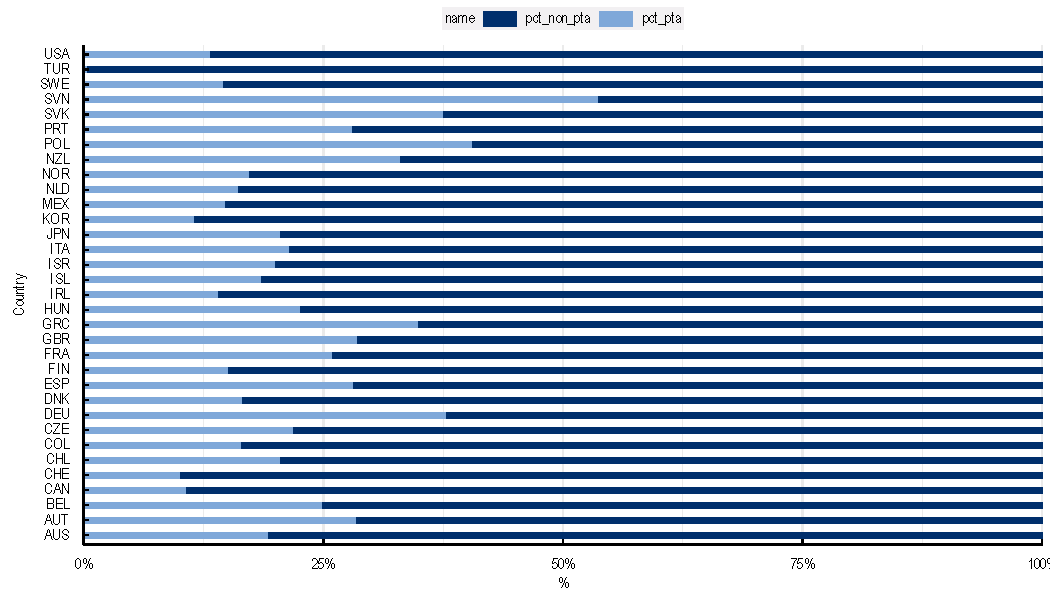
\includegraphics{book_figures/whatif_offmargin_3-1} \end{center}

In this case, we can alter the x-axis scale options to define the range
to go from 0 to 1.01 (or 1.02-1.05).

\begin{Shaded}
\begin{Highlighting}[]
\NormalTok{pta2\_plot }\SpecialCharTok{+}
  \FunctionTok{scale\_x\_continuous}\NormalTok{(}
    \AttributeTok{expand =} \FunctionTok{c}\NormalTok{(}\DecValTok{0}\NormalTok{,}\DecValTok{0}\NormalTok{), }
    \AttributeTok{limits =} \FunctionTok{c}\NormalTok{(}\DecValTok{0}\NormalTok{,}\FloatTok{1.01}\NormalTok{),}
    \AttributeTok{labels =}\NormalTok{ scales}\SpecialCharTok{::}\FunctionTok{percent\_format}\NormalTok{(}\AttributeTok{accuracy =} \DecValTok{1}\NormalTok{)}
\NormalTok{  )}
\end{Highlighting}
\end{Shaded}

\begin{center}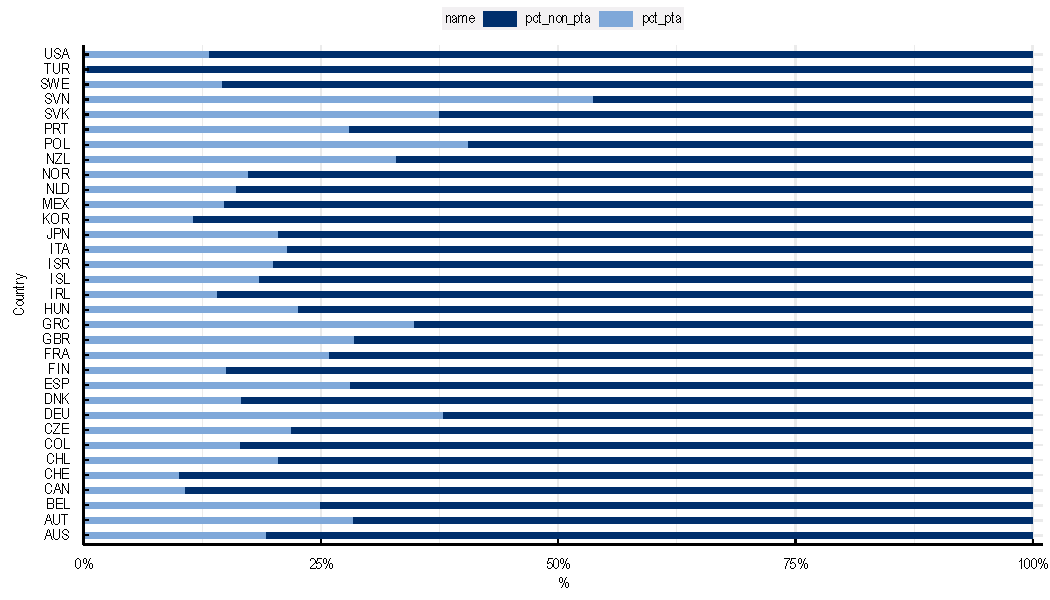
\includegraphics{book_figures/whatif_offmargin_4-1} \end{center}

An alternative solution could be rotating the labels.

\begin{Shaded}
\begin{Highlighting}[]
\NormalTok{pta2\_plot }\SpecialCharTok{+}
  \FunctionTok{theme\_oecd}\NormalTok{(}\AttributeTok{base\_x\_axis\_angle =} \DecValTok{30}\NormalTok{)}
\end{Highlighting}
\end{Shaded}

\begin{center}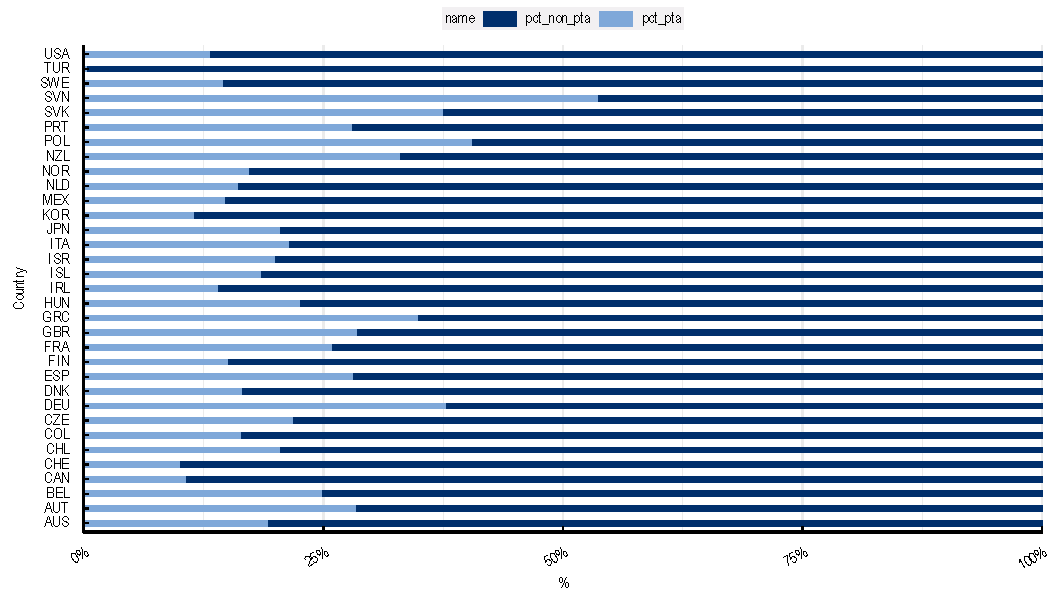
\includegraphics{book_figures/whatif_offmargin_5-1} \end{center}

\hypertarget{too-many-linescolumns}{%
\section{Too many lines/columns}\label{too-many-linescolumns}}

One option is to use ggplot2's \texttt{facet\_wrap()}, as in the next
example.

\begin{Shaded}
\begin{Highlighting}[]
\FunctionTok{ggplot}\NormalTok{(pta }\SpecialCharTok{\%\textgreater{}\%} \FunctionTok{filter}\NormalTok{(country }\SpecialCharTok{\%in\%} \FunctionTok{c}\NormalTok{(}\StringTok{"CAN"}\NormalTok{, }\StringTok{"USA"}\NormalTok{, }\StringTok{"MEX"}\NormalTok{))) }\SpecialCharTok{+}
  \FunctionTok{geom\_col}\NormalTok{(}\FunctionTok{aes}\NormalTok{(}\AttributeTok{x =}\NormalTok{ category, }\AttributeTok{y =}\NormalTok{ pct\_pta), }\AttributeTok{fill =} \FunctionTok{oecd\_clrs}\NormalTok{()[}\DecValTok{1}\NormalTok{]) }\SpecialCharTok{+}
  \FunctionTok{facet\_wrap}\NormalTok{(}\SpecialCharTok{\textasciitilde{}}\NormalTok{country)}
\end{Highlighting}
\end{Shaded}

\begin{center}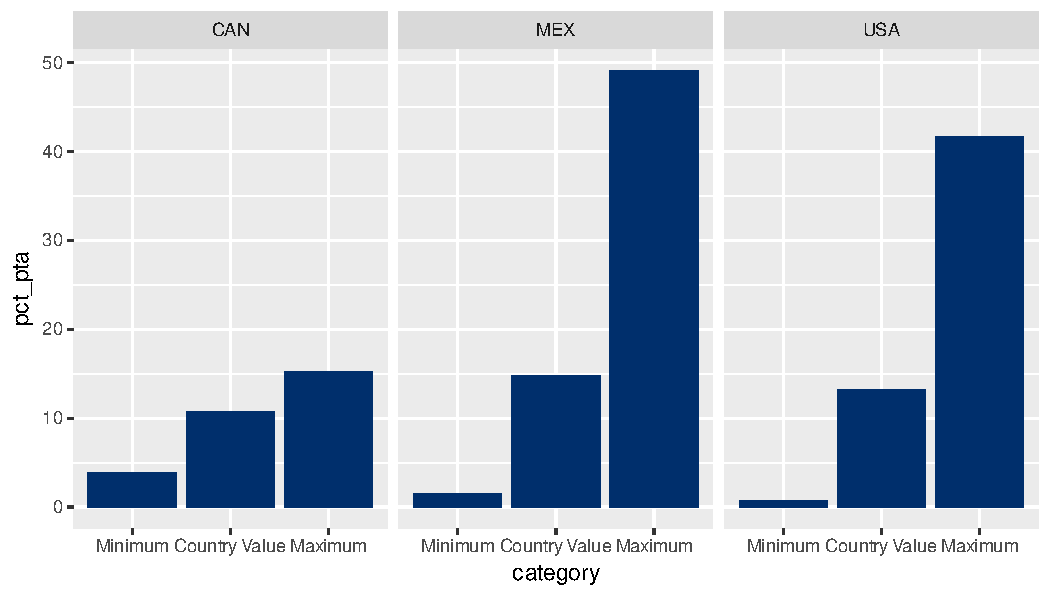
\includegraphics{book_figures/unnamed-chunk-6-1} \end{center}

\newpage

\thispagestyle{empty}
\pagecolor{mypurple}\afterpage{\nopagecolor}

\null
\vfill

\end{document}
